%%%%%%%%%%%%%%%%%%%%%%%%%%%%%%%%%%%%%%%%%%%%%%%%%%%%%%%%%%%%%%%%%%%%%%%%%%%%%%%%%%%%
% Copyright Free Software Lab, 2011                                                %
%                                                                                  %
% Dieses Programm ist freie Software. Sie können es unter den Bedingungen der      %
% GNU General Public License, wie von der Free Software Foundation veröffentlicht, % 
% weitergeben und/oder modifizieren, entweder gemäß Version 3 der Lizenz oder      %
% (nach Ihrer Option) jeder späteren Version.                                      %
%                                                                                  %
% Die Veröffentlichung dieses Programms erfolgt in der Hoffnung, daß es Ihnen      %
% von Nutzen sein wird, aber OHNE IRGENDEINE GARANTIE, sogar ohne die implizite    %
% Garantie der MARKTREIFE oder der VERWENDBARKEIT FÜR EINEN BESTIMMTEN ZWECK.      %
% Details finden Sie in der GNU General Public License.                            %
%                                                                                  %
% Sie sollten ein Exemplar der GNU General Public License zusammen mit diesem      %
% Programm erhalten haben. Falls nicht, siehe <http://www.gnu.org/licenses/>.      %
%%%%%%%%%%%%%%%%%%%%%%%%%%%%%%%%%%%%%%%%%%%%%%%%%%%%%%%%%%%%%%%%%%%%%%%%%%%%%%%%%%%%

%%%%%%%%%%%%%%%%%%%%%%%%%%%%%%%%%%%%%%%%%%%%%%%%%%
% Anfang                                         %
%%%%%%%%%%%%%%%%%%%%%%%%%%%%%%%%%%%%%%%%%%%%%%%%%%
\documentclass[a4paper,11pt,smallheadings,headsepline,titlepage,liststotoc,idxtotoc,bibtotoc,bibliography=totocnumbered]{scrartcl}
\def\ThesisAuthorGivenName{Jan}
\def\ThesisAuthorSurname{Kruska}
\def\ThesisAuthor{\ThesisAuthorGivenName\  \ThesisAuthorSurname}
\def\ThesisAuthorAddress{Grantham Allee 19 \\ 53757 Sankt Augustin}
\def\ThesisExternalCompany{}
\def\ThesisKeywords{}
\def\ThesisLocation{Sankt Augustin}
\def\ThesisPubDate{\today}
\def\ThesisSubject{}
\def\ThesisStudyCourse{Computer Science}
\def\ThesisStudyCourseGerman{Informatik}
\def\ThesisSubjectType{Bachelorarbeit}
\def\ThesisSupervisorFirst{Prof. Dr. Alexander Asteroth}
\def\ThesisSupervisorSecond{Alexander Hagg, M.Sc.}
\def\ThesisSupervisorExternal{}
\def\ThesisTitle{Einbindung von Constraints in eine divergente Optimierungsmethode am Beispiel der Surrogat-assistierten Illumination}
\def\ThesisType{Bachelor}

%\usepackage[table]{xcolor}
\usepackage{aussehen/hbrs-inf}
\usepackage{todonotes}
\usepackage{tabularx}
%\usepackage[utf8]{inputenc}
\usepackage{gensymb}
\usepackage[german]{cleveref}
%\usepackage{dirtree}

\newcommand{\secDir}{abschnitte} % configure section directory

%\newcounter{hypotheses}
%\newcommand{\hypothesis}[1]{
%\label{hyp:abc}
%\begin{itemize}
%	\item[\refstepcounter] 
%\end{enumerate}
%}
\begin{document}
\begin{spacing}{1}
\pagenumbering{roman}


%%%%%%%%%%%%%%%%%%%%%%%%%%%%%%%%%%%%%%%%%%%%%%%%%%
% Deckblatt                                      %
%%%%%%%%%%%%%%%%%%%%%%%%%%%%%%%%%%%%%%%%%%%%%%%%%%
\pagestyle{empty}
\begin{titlepage}
\begin{Large}
\begin{flushleft}
\makebox[11cm][c]{
\parbox[c]{2.5cm}{
\includegraphics[height=4ex]{bilder/fhlogo.pdf}\vspace{1.40cm}}
\parbox[c]{12.0cm}{\begin{flushleft}
\small{\textbf{Hochschule\linebreak{}Bonn-Rhein-Sieg}\linebreak{}\textit{University of Applied Sciences}\linebreak{}\linebreak{}\textbf{Fachbereich \ThesisStudyCourseGerman}\linebreak{}\textit{Department of \ThesisStudyCourse}}
\end{flushleft}}}
\end{flushleft} 
\end{Large}

\vspace{0.150\textheight}
\begin{center}
 \begin{Huge}\textbf{\ThesisSubjectType}\end{Huge}\\
 \vspace{2em}
 \begin{Large}im \ThesisType-Studiengang \ThesisStudyCourse\end{Large}
 \vspace{0.10\textheight}\\
 \begin{Huge} \textbf{\ThesisTitle}
\end{Huge}\\
 \vspace{2em}
 \begin{Large}\textbf{von} \end{Large}\\
 \vspace{1em}
 \begin{Large}\textbf{\ThesisAuthor}\end{Large}\\
\end{center}
\vspace{0.100\textheight}

\begin{Large}
\begin{flushleft}
\begin{tabular}{ll}
Betreuer: & \ThesisSupervisorFirst \\
Zweitbetreuer: & \ThesisSupervisorSecond \\
%Externer Betreuer: & \ThesisSupervisorExternal \\
%~ & \ThesisExternalCompany \\
%~ & \\
Eingereicht am: & \ThesisPubDate
\end{tabular} 
\end{flushleft}
\end{Large}
\end{titlepage}


%%%%%%%%%%%%%%%%%%%%%%%%%%%%%%%%%%%%%%%%%%%%%%%%%%
% Erklärung
%%%%%%%%%%%%%%%%%%%%%%%%%%%%%%%%%%%%%%%%%%%%%%%%%%
\pagestyle{bisHauptteil}
\include{\secDir/Erklärung}

%%%%%%%%%%%%%%%%%%%%%%%%%%%%%%%%%%%%%%%%%%%%%%%%%%
% Inhaltsverzeichnis                             %
%%%%%%%%%%%%%%%%%%%%%%%%%%%%%%%%%%%%%%%%%%%%%%%%%%
\tableofcontents 
\newpage 

%%%%%%%%%%%%%%%%%%%%%%%%%%%%%%%%%%%%%%%%%%%%%%%%%%
% Abbildungsverzeichnis                          %
%%%%%%%%%%%%%%%%%%%%%%%%%%%%%%%%%%%%%%%%%%%%%%%%%%
\listoffigures

%%%%%%%%%%%%%%%%%%%%%%%%%%%%%%%%%%%%%%%%%%%%%%%%%%
% Abkürzungsverzeichnis                          %
%%%%%%%%%%%%%%%%%%%%%%%%%%%%%%%%%%%%%%%%%%%%%%%%%%
%\include{\secDir/Abkürzungsverzeichnis}
\newpage
\end{spacing}

%%%%%%%%%%%%%%%%%%%%%%%%%%%%%%%%%%%%%%%%%%%%%%%%%%
% Einleitung                                     %
%%%%%%%%%%%%%%%%%%%%%%%%%%%%%%%%%%%%%%%%%%%%%%%%%%
\pagestyle{Hauptteil}
\setcounter{page}{1}
\pagenumbering{arabic} 

\clearpage
\section*{Abstract}
Englische Zusammenfassung

\clearpage
\section*{Zusammenfassung}

%Genetische Algorithmen sind ein mächtiges Werkzeug zur Untersuchung komplexer Problemräume. Allerdings stellt die hohe Anzahl an benötigten Funktionsauswertungen ein Problem in solchen Domänen dar in denen die Funktionsauswertung mit erheblichem Rechenaufwand verbunden ist. Durch Surrogat-assistierte Ansätze können die benötigten Funktionsauswertungen um mehrere Größenordnungen reduziert werden, was ermöglicht genetische Algorithmen auch auf solche Problemdomänen anzuwenden. Trotzdem fehlen häufig die Ressourcen für eine multivariate Optimierung, wenn sekundäre Optimierungsziele existieren müssen diese als Constraints in Verfahren eingebunden werden. Die Arbeit untersucht in zwei Problemdomänen, wie Constraints innerhalb des Rahmens der Surrogat-assistierten Illumination, einer phänotypisch divergenten Optimierungsmethode, die MAP-Elites um Surrogat-Assistenz erweitert, verwirklicht werden können.

\section{Einleitung}

Evolutionäre Algorithmen haben sich in der Vergangenheit als mächtige Heuristik zur Untersuchung komplexer Problemräume bewiesen.\todo{Quelle}
Evolutionäre Algorithmen sind dabei in der Lage kreative Lösungen, in komplexesten Problemräumen zu ermitteln.
Genetische Algorithmen sind eine solche Taktik, die an der biologischen Evolution angelehnt entwickelt wurde.
Genetische Algorithmen entwickeln erst eine Möglichkeit eine funktionale Lösung, auch Phänotyp genannt, durch einen Genotypen, was typischerweise ein Vektor eine bestimmten Länge ist, ausdrücken zu können.
Dazu wird eine Funktion benötigt, die diesen Genotypen in einen Phänotypen übersetzt.
Außerdem wird eine Zielfunktion, oder Fitnessfunktion benötigt, mit der die Lösungsqualität eines Individuums, d.h. dessen Phänotyps, ermittelt werden kann.
Sind diese Dinge definiert, können die drei Mechanismen der Evolution, Mutation, Crossover
%\footnote{Manche genetische Algorithmen, wie beispielsweise die $(1+\lambda)$-ES verzichten auf Crossover} und Selektion angewandt werden um eine Population zu Lösung(en) konvergieren zu lassen.
Bei der Anwendung evolutionärer Algorithmen stellen sich allerdings einige Probleme.

Eines dieser Probleme stellt sich recht häufig, da genetische Algorithmen ohne Diversitätsmanagement typischerweise sehr stark konvergieren und dadurch oft in lokalen Optima hängen bleiben.
Um dieser Tendenz entgegenzuwirken und diverse Populationen aufrecht zu erhalten wurden verschiedene Taktiken vorgeschlagen, die sich grob in genotypische und phänotypische Diversitätsmanagementverfahren unterscheiden lassen.
Verfahren zur Erhaltung genotypischer Diversität messen Diversität, die nichts anderes als das Inverse der Ähnlichkeit einer Population untereinander ist, durch die Ähnlichkeit zweier Genotypen zueinander.
Da Genotypen Vektoren sind kann hier auf eines der vielen Ähnlichkeitsmaße, die für Vektoren existieren, zurückgegriffen werden.
Daneben existieren auch solche Verfahren, die Diversität anhand der Ähnlichkeit der Phänotypen messen.
Das hat den Vorteil, das der Phänotyp die Funktion, eines Individuums beschreibt, es wird also funktionale , statt genetischer Diversität hergestellt.
Allerdings bringt dies das weitere Problem mit sich wie man die phänotypische Ähnlichkeit zweier Individuen definiert.
Da der Phänotyp stark von der Problemdomäne abhängt muss diese Ähnlichkeitsdefinition für jede Domäne unterschiedlich erfolgen.
Im Folgenden soll sich mit einer Möglichkeit zum phänotypischen Diversitätsmanagement auseinandergesetzt werden.

Daneben ergeben sich häufig domänenspezifische Probleme.
Eines dieser Probleme ist, dass genetische Algorithmen eine große Zahl von Auswertungen der Fitnessfunktion benötigen.
Das kann dazu führen, dass genetische Algorithmen in Problemdomänen, in denen die Auswertung der Fitnessfunktion rechenaufwändig ist, nicht konkurrenzfähig sind.\todo{komishce formulierung}
Um genetische Algorithmen für solche Probleme nutzen zu können werden somit Möglichkeiten benötigt, die Anzahl an rechenaufwändigen Evaluationen stark zu reduzieren.
Eine solche Möglichkeit die Erfolg gezeigt hat sind Surrogat-Modelle.
Diese werden mit tatsächlichen Evaluationen trainiert, deren Ergebnisse hervorzusagen.
Das führt dazu, dass sie statt der tatsächlichen Evaluation im genetischen Algorithmus genutzt werden können.
Die Auswertung eines Surrogat-Modells benötigt dabei nur einen Bruchteil der Zeit, die eine tatsächliche Evaluation benötigen würde.

Das letzte große Problem, was sich stellt ist die Einbindung von Constraints.
Häufig existieren neben der primären Zielfunktion die optimiert wird, weitere sekundäre Ziele.
Wenn die Ressourcen für eine multivariate Optimierung fehlen, können solche sekundären Optimierungsparameter nicht einfach zu Zielfunktionen erklärt werden.
Stattdessen müssen diese Constraints anderweitig in die Algorithmik eingebunden werden.
Es gibt verschiedene Ansätze zu Integration von Constraints in Optimierungsprobleme, welcher dieser Ansätze aber am Besten funktioniert hängt stark von der Problemdomäne und den Constraints ab.

In dieser Arbeit soll untersucht werden wie sich verschiedene Arten Constraints in die Algorithmik eines divergenten genetischen Verfahren auf die, von diesem Verfahren erzeugten Lösungen, auswirkt.
Dies soll anhand der Lösung eines Problems der Aerodynamik-Domäne durch Anwendung der Surrogat-assistierten Illumination geschehen, einem Verfahren welches den divergenten genetischen Algorithmus MAP-Elites um eine Surrogat-Assistenz erweitert.

% 
%Die Domäne der Aerodynamik stellt eine solche komplexe Problemdomäne dar, deren grundlegende physikalische Regeln zwar verstanden sind, das Zusammenspiel dieser physikalischen Gesetze in der Praxis allerdings so komplex ist, dass häufig auf allgemeine Faustregeln zum aerodynamischen Design zurückgefallen wird.
%Sowohl bei der allgemeinen genetischen Programmierung, als auch bei der konkreten Anwendungsdomäne stellen sich dabei einige Probleme.
%Eines dieser Probleme ist Diversitätsmanagement.
%Um nicht in lokalen Optima stecken zu bleiben wird häufig Taktiken zum Diversitätsmanagement eingesetzt.
%

%\subsubsection{Abbildungen}
%\begin{figure}[!ht]
%  \begin{center}
%    
\includegraphics[width=3cm]{bilder/fhlogo.pdf}
%    \caption{Logo Hochschule Bonn-Rhein-Sieg}
%    \label{an_tranciver}
%  \end{center}
%\end{figure}
%
%\begin{figure}[!ht]
%  \begin{center}
%    
\includegraphics[width=3cm]{bilder/fhlogo.pdf}
%    \caption{Logo Hochschule Bonn-Rhein-Sieg}
%    \label{an_tranciver}
%  \end{center}
%\end{figure}
%
%\begin{figure}[!ht]
%  \begin{center}
%    
\includegraphics[width=3cm]{bilder/fhlogo.pdf}
%    \caption{Logo Hochschule Bonn-Rhein-Sieg}
%    \label{an_tranciver}
%  \end{center}
%\end{figure}
%
%\begin{figure}[!ht]
%  \begin{center}
%    \begin{tabular}{|c|c||c|c|c|c|c|c|c|c|c||c||c|c|}
%    \hline
%    P & Q & $\neg$ & ( P & $\vee$ & Q ) & $\vee$ & ( $\neg$ & P & $\wedge$ & Q ) & $\equiv$ & $\neg$ & P  \\ \hline \hline
%    0 & 0 & 1 & 0 & 0 & 0 & $\mathbf{1}$ & 1 & 0 & 0 & 0 & & $\mathbf{1}$ & 0\\ \hline
%    0 & 1 & 0 & 0 & 1 & 1 & $\mathbf{1}$ & 1 & 0 & 1 & 1 & & $\mathbf{1}$ & 0\\ \hline
%    1 & 0 & 0 & 1 & 1 & 0 & $\mathbf{0}$ & 0 & 1 & 0 & 0 & & $\mathbf{0}$ & 1\\ \hline
%    1 & 1 & 0 & 1 & 1 & 1 & $\mathbf{0}$ & 0 & 1 & 0 & 1 & & $\mathbf{0}$ & 1\\ \hline
%    \end{tabular}
%    \caption{Wahrheitstabelle: $\neg$ ( P $\vee$ Q ) $\vee$ ( $\neg$ P $\wedge$ Q ) $\equiv$ $\neg$ P}
%  \end{center}
%\end{figure}
%
%\subsection{Zitate}
%\cite{BarAhl08} sagen hier steht ein Text. \\
%\citet{BruMurPerWygMcN09} sagen hier steht ein Text. \\
%\citet*{BruMurPerWygMcN09} sagen hier steht ein Text. \\
%"`Hier steht ein Text."' \citep{BarAhl08} \\
%Hier steht ein Text. \citep[Vgl.][]{BarAhl08} \\
%Hier steht ein Text. \citep[][S. 200]{BruMurPerWygMcN09} \\
%Hier steht ein Text. \citep*[][S. 200]{BruMurPerWygMcN09} \\
%Hier steht ein Text. \citep{wiki:001,BruMurPerWygMcN09} \\
%
%
%\subsubsection{Abkürzungen}
%\acf{GSM} \\
%\acs{NUA} \\
%\acl{BUT}  \\
%\acp{UA} \\
%
%
 

%%%%%%%%%%%%%%%%%%%%%%%%%%%%%%%%%%%%%%%%%%%%%%%%%%
% Stand der Forschrung                           %
%%%%%%%%%%%%%%%%%%%%%%%%%%%%%%%%%%%%%%%%%%%%%%%%%%
\newpage
\section{Grundlagen}
\label{sub:grundlagen}
\subsection{Genetische Algorithmen}

Genetische Algorithmen sind eine Klasse von Optimierungsalgorithmen, die sich an den Mechanismen der natürlichen Evolution orientieren\cite{Simon.2013}.
Namentlich Mutation, Crossover und Selektion.
Die Begrifflichkeiten orientieren sich entsprechen an der natürlichen Evolution.
Genetische Algorithmen arbeiten typischerweise mit Populationen aus Individuen, welche sich über Generationen entwickeln.
Jedes Individuum besitzt einen Genotypen sowie einen Phänotypen.
\missingfigure{Vllt. Bild geno phäno}
Der Genotyp eines Individuums ist typischerweise ein Vektor, das Genom des Individuums genannt, der aus einzelnen Zahlen, den Genen des Individuums, besteht. Dieser stellt die genetischen Informationen eines Individuums dar. Daneben existiert in genetischen Algorithmen eine Mapping-Funktion mit der eine Genotyp in einen Phänotyp, der nichts anderes als eine konkrete Lösung des Optimierungsproblems ist, übersetzt werden kann.

\begin{algorithm}
\caption{Genetischer Algorithmus} \label{alg:geneticAlgorihtm}
\begin{algorithmic}[1]
	\Procedure{GeneticAlgorithm}{$fitnessFunction,hyperparameters$}
	\State $population \gets initializePopulation$
	\State $populationFitness \gets fitnessFunction(population)$
	\For{$numberIterations$}
		\State $children \gets crossover(population,hyperparameters)$
		\State $children \gets mutate(children,hyperparameters)$
		\State $childFitness = fitnessFunction(children)$
		\State $population \gets selection(population,populationFitness,children,childFitness)$
		\State $populationFitness \gets updateFitness(population)$
	\EndFor
	\EndProcedure
\end{algorithmic}
\end{algorithm}

Die Mechanismen der Mutation und des Crossovers agieren auf der Ebene des Genotyps.
Mutation beschreibt die Situation, dass sich jedes Gen mit einer bestimmten Wahrscheinlichkeit ändern kann. 
Abhängig vom Typen des Gens, ist eine Änderung unterschiedlich formuliert, eine reelle Zahl mag sich anhand einer Normalverteilten Zufallsvariable ändern, eine natürliche Zahl mit $\pm1$ und ein Index mag einen zufälligen möglichen Index annehmen. 
Mutatation ist für einen genetischen Algorithmus wichtig, da sich durch diese neue Eigenschaften entwickeln können.

Crossover beschreibt die Situation, dass zwei oder mehr Elternindividuuen zu einem Kindindividuum kombiniert werden. 
Auch hier ist keine konkrete Implementierung nicht vorgeschrieben, wichtig ist nur, dass ein Kind als Kreuzung der Eltern erzeugt werden kann.
Das Ziel des Crossovers ist es, dass sich positive Eigenschaften in Populationen verteilen und mehrere unabhängig entstandenen positiven Mutationen in einem Individuum vereint werden.
Es ist allerdings anzumerken, dass Crossover einen optionalen Teil von genetischen Algorithmen darstellt, einige Algorithmen%, wie beispielsweise ($1 + \lambda$)-ES 
verzichten aus verschiedenen Gründen auf Crossover und mutieren ihre Populationen nur.
Diese beiden Methoden stellen sicher, dass neue Genotypen, und damit neue Lösungen generiert werden können, stellen aber keine Mechanismus zur Verfügung durch den dem Algorithmus eine Optimierungsrichtung gegeben wird.

Der Mechanismus, der der Optimierung eine Richtung gibt ist die Selektion.
Anders als die ersten beiden agiert diese auf Phänotypen, sprich ausgedrückten Lösungen.
Jeder genetische Algorithmus benötigt eine Funktion mit der Lösungen bewertet werden können.
Dies kann entweder in Form einer Fitnessfunktion, die die Güte eines Individuums berechnet, bei der höhere Werte besser sind, oder in der Form einer Kostenfunktion, die die Kosten eines Individuums berechnet und bei der entsprechend niedrigere Werte besser sind, geschehen.
Ob eine Fitness- oder Kostenfunktion genutzt wird hängt von der Problemformulierung ab, und ist letztendlich nur eine Frage der Algorithmus minimiert oder maximiert.
Mit diesen Funktionen kann für jedes Individuum eine Qualität berechnet werden, und Individuen können bezüglich dieser verglichen werden.
Durch Selektion werden in jeder Iteration dann schlechte Lösungen eliminiert, wodurch die Population sich zu Optima hinbewegt.
%Die Fitness, bzw. der Kosten jedes Individuums kann dann ermittelt werden und die Selektion eliminiert dann schlechte Lösungen, sprich solche mit niedriger Fitness, bzw. hohen Kosten.
Selektion ist häufig nicht so simpel, dass einfach die besten Individuen ausgewählt werden.
Die in \ref{sub:divergetnGeneticAlgorithms} besprochenen Ansätze zum Diversitätsmanagement, berücksichtigen Diversität von Populationen und können diverse Lösungen bevorzugt auswählen.

In der Gesamtschleife werden also in jeder Generation per Crossover Kinder erzeugt, die daraufhin mutiert werden.
Für diese Kinder wird dann eine Fitness berechnet.
Daraufhin werden durch die Selektion die besten Individuen ermittelt, welche zur nächste Elterngeneration werden.
Diese Schleife wird solange wiederholt bis das Maximum an Generationen erreicht ist.

\subsubsection{Divergente genetische Algorithmen}

\label{sub:divergentGeneticAlgorithms}

Eine sehr häufige Anforderung an genetische Algorithmen ist die Einbindung von Divergenz, bzw. Diversität.
Dies hat verschiedene Gründe.
Einerseits führt eine niedrige Diversität der Individuen dazu, dass nur ein kleiner Bereich des Suchraums, nämlich der in dem die Individuen liegen abgesucht wird.
Sehr homogene Populationen können dadurch einfach in lokalen Optima stagnieren, da andere Optima zu weit im Suchraum entfernt sind.
In einer diversen Population ist das Springen aus lokalen Optima hingegen einfacher, und selbst wenn Populationen stagnieren, dann geschieht dies in mehreren Optima gleichzeitig, wodurch die Wahrscheinlichkeit in einem im globalen Vergleich gutes lokalen Optimum zu finden steigt.
Auch ist es nicht unbedingt wünschenswert eine sehr homogene Population als Ergebnis zu erhalten, da die Individuen mit hoher Wahrscheinlichkeit aller der gleichen Lösungsklasse angehören.
Wenn man eine diverse Population aus Individuen erhält können Aussagen über unterschiedliche Lösungsklassen getroffen werden, Lösungsklassen und ihre Qualität können miteinander verglichen werden, und je nachdem kann größere Erkenntnis erlangt werden, was eine qualitativ hochwertige Lösung ausmacht wodurch wiederum das gestellte Problem besser verstanden werden kann.

Es existieren verschiedenste Ansätze um Diversität zu gewährleisten, welche sind grundsätzlich in genotypische und phänotypische Ansätze aufteilen lassen, abhängig davon wo Diversitätsmanagement stattfindet.
Ansätze wie Niching\cite{Shir.2012}, gewährleisten genotypische Diversität durch die Ermittlung der genetischen Ähnlichkeit zweier Individuen.
Das hat den Vorteil, dass der Genotyp eines Individuums typischerweise ein Vektor ist, und eine Vielzahl von Ähnlichkeitsmetriken für Vektoren existiert.
Dadurch fällt die Definition, was Diversität ausmacht sehr leicht.
Auch ist die Berechnung einer Distanz zwischen Vektoren sehr effizient, was vorteilhaft ist, da die Berechnung von Diversität typischerweise sehr häufig stattfinden muss.
Allerdings hat es den Nachteil, dass, besonders wenn die Genotyp-zu-Phänotyps-Mapping Funktion komplex ist, genetische Distanz nicht funktionaler Distanz zwischen Lösungen enspricht.
D. h. es besteht die Möglichkeit, dass genetisch unähnliche Individuen trotzdem in die gleiche Lösungsklasse fallen.
Deshalb wurden Ansätze wie Novelty-Search\cite{Lehman.2011} oder MAP-Elites\cite{Mouret.4202015} zum Diversitätsmanagement vorgeschlagen, die Diversität auf der Ebene, des Phänotyps bestimmen und somit funktionale Distanz messen.
Da der Phänotyp domänenspezifisch,  muss die Diversitätsmetrik für jede Domäne maßgeschneidert definiert werden, und es kann nicht auf Allgemeinlösungen zurückgegriffen werden.
Auch besteht eine erhebliche Limitierung bezüglich der Komplexität einer solche Diversitätsmetrik, da die Diversität typischerweise sehr häufig berechnet werden muss.

\subsubsection{MAP-Elites}

\label{sub:mapElites}
\begin{algorithm}
	\caption{MAP-Elites} \label{alg:mapElites}
	\begin{algorithmic}[1]
		\Procedure{MapElites}{$fitnessFunction,categorizationFunction,hyperparameters$}
		\State $map \gets $ \Comment{Initialize empty n-dimensional map}
		\State $fitness \gets $ \Comment{Initialize empty n-dimensional fitnessMap}
		\State $population \gets initializeRandomPopulation$ \Comment{Start of with randomly generated intitial samples}
		\For{$individual in population$}
			\State $f = fitnessFunction(individual)$
			\State $c = categorizationFunction(individual)$ \Comment{Categorization c is an Index to a cell in the map}
			\If{$map(c) = \emptyset \lor f < fitness(c)$} \Comment{If cell is unoccupied or this solution is better put it in cell}
				\State $map(c) \gets individual$
				\State $fitness(c) \gets f$
			\EndIf
		\EndFor
		
		\For{$numberGenerations$}
			\State $children \gets selectRandom(population,childrenPerGeneration)$ \Comment{Select samples randomly from existing solutions}
			\State $children \gets variate(children,hyperparameters)$ \Comment{Variate these children with crossover and/or mutation}
			\For{$individual in children$}
				\State $f = fitnessFunction(individual)$
				\State $c = categorizationFunction(individual)$
				\If{$map(c) = \emptyset \lor f < fitness(c)$}
					\State $map(c) \gets individual$
					\State $fitness(c) \gets f$
				\EndIf
			\EndFor
		\EndFor
		\Return $map,fitness$
		\EndProcedure
	\end{algorithmic}
\end{algorithm}
MAP-Elites (Multi-dimensional Archive of Phenotypic Elites)\cite{Mouret.4202015} ist ein genetischer Algorithmus mit phänotypischem Diversitätsmanagement.
Das bedeutet, dass die Morphologie bzw. Funktionalität einer konkreten ausgedrückten Lösung, wie beispielsweise Volumen oder Krümmung eines Bauteils, betrachtet wird.
Dazu wird der Lösungsraum entlang anhand beliebig vieler Features, deren Untersuchung als zielführend zum Verständnis des Problems befunden wird, aufgeteilt.
Diese Feature Dimensionen sind direkte Merkmale der Phänotypen von Lösungen, wie beispielsweise das Volumen eines Phänotypos in einer dreidimensionalen Domäne.
Als Features sollten solche Merkmale gewählt werden die unabhängig von der Zielfunktion sind, d. h. deren Einfluss auf die Fitness von Lösungen unklar ist.
Gerade die Untersuchung wie Merkmale mit der Fitness interagieren ist ein typisches Untersuchungsziel für MAP-Elites.
Diesen Feature-Dimensionen wird ein Minimum, Maximums sowie eine Schrittweite zugewiesen um den Lösungsraum in Zellen zu diskretisieren.
Diese Diskretisierung zu Zellen wird typischerweise Karte oder Archiv genannt.
Wichtig für MAP-Elites ist das jede Zelle nur maximal eine Lösung enthalten kann.
%Jede dieser Zellen stellt dabei eine Kombination der Eigenschaften dar.
Zu Beginn des Algorithmus werden alle Zellen leer initialisiert, im Laufe des Algorithmus werden diese nach und nach gefüllt.
Zuerst werden zufällige Individuen generiert um die Karte mit einer Initialpopulation zu befüllen.
Daraufhin werden in jeder Generation aus den momentan in der Karte enthaltenen Lösung zufällig Individuen ausgewählt um die Kindpopulation zu erzeugen.
Aus dieses ausgewählten Individuen wird eine Kindpopulation per Mutation und/oder Crossover erzeugt.
Jedes dieser Kinder wird bezüglich dessen Fitness evaluiert und dessen zugehöriger Phänotyp wird nach den gewählten Features kategorisiert.
Diese Kategoriesierung weist jedem Kind eine Zelle zu die es befüllen könnte.
Ist diese Zelle noch leer befüllt das Kind diese, befindet sich bereits ein Individuum in der Zelle, findet zwischen diesem und dem Kind lokal Konkurrenz statt.
Die lokale Konkurrenz innerhalb der Zellen ist was MAP-Elites zu einem divergenten Algorithmus macht.
Da Lösungen nur durch Lösungen verdrängt werden können, denen die gleiche Zelle zugewiesen ist, können Lösungen nur durch ihnen phänotypisch ähnliche Lösungen verdrängt werden.
Dadurch wird die phänotypische Diversität des Algorithmus gewährleistet.
Außerdem kann die Größe des Archivs während des Algorithmus nur zunehmen, da Individuen nur verdrängt werden können wenn sie durch ein anderes ersetzt werden, aber im Laufe des Algoithmus immer mehr leere Zellen befüllt werden können.
Dass bedeutet, dass die Anzahl an lokalen Optima, die der Algorithmus ermittelt hat über dessen Laufzeit wächst.

%Dadurch ist der Algorithmus divergent, denn dadurch, dass nur lokale Konkurrenz stattfindet kann ein Individuum nur durch ein phänotypisch ähnliches verdrängt werden, wodurch die phänotypische Diversität nicht sinkt.
Nicht nur wird eine Vielzahl von Lösungen generiert, die unterschiedliche Lösungsklassen abdecken, sondern die regelmäßig aufgeteilte Karte kann auch dabei helfen die Effekte, die die Features auf die Lösungsqualität haben zu verstehen.


\subsection{Surrogat-Modellierung}

\label{sub:surrogate}
Für die Selektion von Individuen innerhalb eines genetischen Algorithmus wird die Lösungsqualität dieser Individuen, typischerweise Fitness genannt, benötigt.
Durch die große Anzahl an Individuen die für den evolutionären Algorithmus benötigt werden, findet die Auswertung der Fitnessfunktion sehr häufig statt.
Dies stellt bei relativ einfachen Fitnessfunktionen keine große Einschränkung dar, auf Problemdomänen in denen die Auswertung der Fitness eines Individuums allerdings komplexer und dadurch zeitaufwändiger wird, kann dies die Anwendbarkeit einfacher genetischer Algorithmen einschränken.

Aerodynamische Probleme, für die zeitaufwändige Simulationen nötig sind, gehören ohne Zweifel zu der Klasse von Problemen, für die die Anzahl der benötigten Funktionsauswertungen zu groß sind, als das der Algorithmus in vertretbarer Laufzeit abschließen kann.
Um genetische Taktiken auf eine solche Problemdomäne anzuwenden, wird eine Möglichkeit benötigt die benötigten Funktionsauswertungen erheblich zu reduzieren.
Eine solche Möglichkeit ist ein Surrogatmodell \cite{Jin.2011}\cite{Preen.2016}, eine Machine-Learning Modell, welches aufgrund echter Simulationsauswertungen trainiert wird, um deren Ergebnis annähernd vorherzusagen.
Eine Auswertung des Modells erfordert dabei nur einen winzigen Bruchteil des Aufwands, der für eine Simulation nötig wäre.

Die Einführung eines Surrogatmodells bringt allerdings einige Probleme mit sich.
Das wichtigste zu lösende Problem ist, wie bestimmt wird anhand welcher realen Funktionsauswertungen das Surrogatmodell trainiert wird.
Dabei müssen einige Ziele beachtet werden.
Ersten sollte das Surrogatmodell möglichst präzise sein, da es seinen Zweck für reale Funktionsauswertungen einzustehen nur erfüllen kann, wenn die Vorhersagen des Surrogatmodells ausreichend gut reale Funktionauswertungen abbilden.
Da das Surrogatmodell aber genau für den Zweck genutzt wird die Anzahl an benötigten teuren Funktionsauswertungen zu reduzieren, wäre es sinnvoll, wenn Funktionauswertungen so gewählt werde, dass sie maximalen Nutzen bringen.


\subsubsection{Gaußprozesse}

\missingfigure{Visualisierung Gaußprozess}

\todo{Mehr Gaußprozess ausführen}
Gaußprozesse sind ein in \cite{Rasmussen.2008} entwickeltes Machine-Learning Verfahren, mit welchem beliebige mathematische Funktionenen approximiert werden können. 
Ein großer Vorteil von Gaußprozessen ist, dass sie durch ihre Herkunft aus der Statistik die zu approximierende Funktion als Kombination aus Normalverteilungen modellieren.
Dadurch können Gaußprozesse neben einer Vorhersage, genauer gesagt dem Mittelwert der Vorhersage an einem Punkt, auch die Varianz der Vorhersage an jedem Punkt liefern.
Durch diese Eigenschaft bieten sie gute Vorraussetzungen zur Anwendung von Upper-Confidence-Bound, und können dadurch Vorhersagen welche Funktionsauswertungen den statistisch höchsten Nutzen unter Abwägung zwischen Exploration und Exploitation haben.
Damit können die benötigten Funktionsauswertungen weiter reduziert werden, beziehungsweise die Präzision des Modells bei begrenzter Zahl von Funktionsauswertungen maximiert werden.
Diese Eigenschaft stellt den Hauptvorteil von Gaußprozessen gegenüber anderen Machine-Learning Verfahren dar und ist der Grund warum Gaußprozesse als Surrogatmodell in SAIL genutzt werden.

%Dies ist für die Nutzung als Surrogatmodell genau deshalb wünschenswert, da es ein Maß der Präzision für jeden Punkt der Funktion darstellt.
%Da die Auswertung eines Punktes und die Einführung dieses in den Gaußprozess, immer den Kollaps der Varianz an diesem Punkt zu null zu Folge hat, bietet der Gaußprozess eine Möglichkeit den Präzisionsgewinn durch die Auswertung eines Punktes zu quantifizieren.


Der Hauptnachteil von Gaußprozessen ist die relativ hohe Speicher- und Rechenkomplexität, da die Anzahl an Simulationen die durchgeführt werden können aber ohnehin durch den Rechenaufwand, der mit diesen verbunden, ist, stark limitiert ist, wird die Anzahl an Trainingsdaten so gering bleiben, dass Komplexitätsüberlegungen hinfällig sind.

\subsubsection{Exploration Exploitation Problem}

Ein häufig auftretendes Dilemma, wenn der Gewinn eines unbekannten Problems maximiert werden soll, ist die Spannung zwischen Exploration und Exploitation.
Das einfachste Beispiel in dem eine solche Spannung existiert ist das Problem des mehrarmigen Banditen.
In diesem Problem existiert eine Reihe von Glücksspielautomaten, deren Gewinn durch statistische Verteilungen beschrieben wird.
Der Gewinn jedes einzelnen Automaten wird durch eine andere Verteilung definiert.
Diese Verteilungen sind einem Spieler, der das Ziel hat seinen Gewinn zu maximieren, allerdings nicht bekannt.
Mit jedem Spiel an einem Automaten erhält der Spieler sowohl den Gewinn des Spiels, als auch Wissen über die Gewinnverteilung des Automaten und damit über das gesamte Problem.
Das Problem ist die Frage mit welcher Strategie der Spieler seinen Gewinn maximieren kann.
Der Spieler kann nur den Automaten Spielen der den besten bekannten erwarteten Gewinn hat, allerdings besteht die Möglichkeit, dass ein anderer unbekannter Automat einen höheren erwarteten Gewinn besitzt, von dem der Spieler allerdings nicht weiß.
Stattdessen kann der Spieler versuchen Wissen über das Problem zu sammeln indem er an Automaten spielt über deren Verteilung er wenig weiß. 
Dies führt aber dazu, dass der Spieler an vielen schlechten Automaten spielen wird um mehr Wissen über diese zu erlangen.
Das Dilemma zwischen diesen Entscheidungen ist ein Beispiel Exploration Exploitation Problem.
An dem besten bekannten Automaten zu spielen ist ein Beispiel der Exploitation, der Ausnutzung des Wissens, an unbekannten Automaten zu spielen ein Beispiel der Exploration, der Sammlung von Wissen.

Allgemeiner formuliert beschreibt Exploration dabei die Untersuchung von unbekannten, bisher unerforschten Gebieten, um das zugrundeliegende Problem besser zu verstehen und damit Strategien besser optimieren zu können, während Exploitation die Ausnutzung des gesammelten Wissens beschreibt um den Nutzen zu maximieren.
Die beiden Herangehensweisen stellen gegensätzliche Konzepte dar.
Je mehr Exploration durchgeführt wird, desto weniger Exploitation kann durchgeführt werden und vice-versa.

Ein solches Problem stellt sich auch bei der Surrogatmodellierung.
So ist einerseits die Exploration unerkundeter Gebiete wichtig um die globale Präzision des Modells zu maximieren und Optima in unerforschten Bereichen zu finden.
Andererseits ist die Exploitation wichtig um Regionen um lokale Optima möglichst präzise abzubilden, da in diesen Regionen der Hauptteil der Optimierung stattfindet.
Ist das Surrogatmodell in Regionen hoher Fitness nicht präzise, beschränkt das die maximale Qualität der Lösungen, die der Optimierungsalgorithmus, der auf das Surrogatmodell zurückgreift, erzeugen kann.
Außerdem ist die Anzahl an erlaubten realen Auswertungen stark begrenzt, die Reduzierung dieser ist der Grund für die Nutzung eines Surrogatmodells.
D. h. dass die Auswertungen, die durchgeführt werden maximalen Nutzen für das Surrogatmodell haben sollten.

\missingfigure{UCB}
Eine Möglichkeit mit dem Dilemma zwischen Exploration und Exploitation umzugehen ist das in \cite{Auer.2002} beschriebene Upper-Confidence-Bound. Dabei werden Exploration-Exploitation Probleme als statistischen Prozesse bestehend aus Mittelwert und Varianz aufgefasst.
Der Mittelwert an einem Punkt spiegelt dabei den erwarteten Nutzen wieder, eine dem Mittelwert folgende Auswahl bevorzugt also Exploitation von Bereichen in denen der erwartete Nutzen hoch ist.
Die Varianz spiegelt die Unsicherheit an einem Punkt wieder, eine Auswahl nach Varianz bevorzugt die Exploration von Bereichen in denen eine hohe Varianz auftritt, oder anders gesagt von bisher unerforschten Bereichen.
Upper-Confidence-Bound kombiniert Mittelwert und Varianz zur Bestimmung der besten Punkte, und erreicht damit eine Balance in der sowohl Exploration als auch Exploitation stattfindet.

%Durch die Auswertung von Punkten mit hoher Varianz kann die Anzahl an benötigten realen Funktionsauswertungen gering gehalten werden.
%Die Auswertung von Punkten mit hoher Varianz, sprich die Auswertung von bisher nicht erkundeten Gebieten wird Exploration genannt.
%Wenn allderdings nur die Exploration des Suchraums durchgeführt wird, wird dies dazu führen, dass viele nicht-optimale Bereiche erkundet werden.
%Da der Gaußprozess im Kontext einer Optimierung genutzt wird hat die Präzision des Gaußprozesses in Bereichen um Optima besondere Bedeutung.
%Die Verbesserung der Präzision des Gaußprozesses in optimalen Regionen wird Exploitation genannt.
%Insgesamt muss eine Abwägung zwischen der Exploration unbekannter Bereiche der Funktion und der Exploitation bekannter optimaler Bereiche der Funktion stattfinden. 
%Eine Möglichkeit einer solchen Abwägung ist Upper-Confidence-Bound \todo{cite}, einer Kombination aus Mittelwert, der Exploitation bevorzugt, und Varianz, die Exploration bevorzugt.

\subsubsection{SAIL}

\begin{algorithm}
	\caption{MAP-Elites} \label{alg:mapElites}
	\begin{algorithmic}[1]
		\Procedure{MapElites}{$evaluate,categorizationFunction,hyperparameters$}
			\While{$numberEvaluatedSamples < totalSamples$}
				\If{$notInitialized$}
\State $evaluatedSamples \gets evaluate(randomSampling())$ \Comment Evaluate is the real costly Fitness-Function.
\Else
\State $surrogate \gets trainSurrogate(evaluatedSamples)$
\State $acquisitionMap \gets MapElites(acquisitionFunction,categorizationFunction,hyperparameters)$
\State $nextSamples \gets sampleRandomFromMap(acquisitionMap)$ \Comment SAIL utilizes Sobol-sequences to achieve optimal spread of the Sampling
\State $evaluatedSamples \gets evaluatedSamples \cup evaluate(nextSamples)$
\EndIf
			\EndWhile
		\EndProcedure
	\end{algorithmic}
\end{algorithm}

\missingfigure{Vllt. Graphik zu SAIL}

SAIL (Surrogate-Assisted Illumination) ist ein in \cite{Gaier.6152018} beschriebenes Verfahren, welches die in \ref{sub:mapElites} und \ref{sub:surrogate} beschriebenen Ansätze vereint, mit dem Ziel MAP-Elites in rechenintensiven Domänen anwendbar zu machen.

Zur Initialisierung SAILs werden zuerst zufällig Samples ausgewählt und evaluiert.
Um eine gleichmäßige Verteilung der Samples über den Problemraum zu garantieren werden diese Samples nicht aus einer Gleichverteilung, sondern aus einer Sobol Sequenz ausgewählt.\todo{Ausführen sobol sequenz}
Der eigentliche Kern von SAIL ist die graduelle Verfeinerung des Surrogatmodells.
In jeder Iteration der Verfeinerungsschleife wird ein Gaußprozess auf Basis aller bisher ausgewerteten Samples trainiert.
Mit diesem Gaußprozess wird MAP-Elites durchgeführt, wobei als Fitnessfunktion für die Durchführung von MAP-Elites die Akquisefunktion genutzt wird.
Dadurch wird die sogenannte Akquisekarte erzeugt, welche diverse Lösungen enthält, die die Akquisefunktion maximieren.
Aus dieser Akquisekarte werden dann mehrere Lösungen für reale Fitnessevaluationen ausgewählt.
Durch die Nutzung von Upper-Confidence-Bound als Akquisefunktion stellen diese Lösungen Optima bezüglich Exploration und Exploitation dar.
Die ausgewählten Samples werden daraufhin ausgewertet  und den bereits ausgewerteten hinzugefügt um den Gaußprozess in der nächten Iteration besser zu trainieren.
Dies kann abhängig von den verfügbaren Rechenkapazitäten beliebig oft wiederholt werden.
Am Ende poduziert diese Schleife eine Menge an echten Ausgewerteten Samples auf deren Basis der Gaußprozess trainiert werden kann.

Um am Ende Ergebnisse zu erzeugen kann MAP-Elites mit dem finalen Gaußprozess und dessen Mittelwert als Fitnessfunktion ausgeführt werden.
Der Mittelwert des Gaußprozesses an einem Punkt entspricht gerade der mittleren Vorhersage zur Fitness einer realen Auswertung an diesem Punkt.
Damit wird dann eine diverse Vorhersagekarte erzeugt, die die Optima des Gaußprozesses zeigt.
Bei korrekter Parametrisierung von SAIL, dem Gaußprozess, und einer ausreichen großen Anzahl an realen Auswertungen korrespondieren OPtima im Gaußprozess mit Optima in der realen Fitnessfunktion.

In \cite{Gaier.6152018} wurde gezeigt, dass dieser Ansatz erfolgreich auf 2D und 3D aerodynamische Domänen angewandt werden kann.
Dort wurden per Freiform-Deformation dreidimensionale Objekte deformiert.
Da die Auswertung der Fitnessfunktion in der Auswertung einer aerodynamische Simulation bestand wurde ein Surrogatnetzwerk genutzt.


\subsection{Constraints in Optimierungsprozessen}
Constraints sind eine Möglichkeit sekundäre Optimierungsparemter, welche neben dem primären Optimierungsziel ebenfalls eingehalten werden sollen, in einen Optimierungsprozess einzuarbeiten, ohne auf multivariate Optimierung zurückgreifen zu müssen.
Constraints lassen sich grundsätzlich in Soft Constraints, bei denen die Nichteinhaltung des Constraints zur Addition von Strafwerten auf die Optimierungsfunktion führt, und Hard Constraints, die eine binäre erfüllt/nicht erfüllt Auswahl treffen.
Welche dieser beiden Arten von Constraints genutzt wird, hängt stark von der Problemstellung ab.

Auch stellt die Formulierung von Constraints häufig eine Herausforderung dar.
So müssen diese offensichtlich berechenbar sein, Constraints sind allerdings häufig nicht in mathematischer Form formuliert sondern eher in einer Art die an Requirements erinnert.
Es muss folglich zuerst eine mathematische Formulierung für den Constraint entwickelt werden, die den Constraint soweit wie möglich entspricht.
Zweitens werden Constraints in einem typischen evolutionären Optimierungsalgorithmus sehr häufig evaluiert werden. Das bedeutet, dass die Berechnung des Constraints entweder nicht besonders rechenintensiv sein darf, oder Hilfsmechanismen integriert werden wie beispielsweise die Modellierung des Constraint durch ein Surrogatnetzwerk, wie es in SAIL für die Fitness bereits genutzt wird.

\subsubsection{Ausschluss durch Definition der Repräsentation}

Die einfachste Art mit äußeren Einschränkungen umzugehen, ist es die Repräsentation des Problems so zu formulieren, dass es nicht möglich ist Phänotypen zu generieren, die den Constraint verletzen.
Im Gegensatz zum Phänotyp, dessen Definition von der Problemdomäne abhängt, kann der Genotyp frei definiert werden.
Die einzigen Kriterien die dieser Erfüllen muss sind, dass eine Abbildung existiert mit der aus einem Genotyp ein zugehöriger Phänotyp generiert werden kann, dass die Methoden der evolutionären Optimierung, sprich Mutation und Crossover, mit ihm durchgeführt werden, und dass neue zufällige Genotypen generiert werden können.
Die Wahl einer guten Repräsentation des Problems ist einer der wichtigsten Teile der evolutionären Optimierung.
So existieren Beispiele, in denen das gleiche Problem mit einer Repräsentation nicht gelöst werden kann, während dies mit einer anderen Repräsentation möglich ist.
Constraints können in der Wahl der Problemrepräsentation bereits behandelt werden.
Ist es möglich, durch eine kluge Wahl der Repräsentation zu garantieren, dass nur solche Genotypen generiert werden können deren zugehöriger Phänotyp den Constraint erfüllt, ist sichergestellt, dass jede mögliche Lösung valide ist, und der Constraint nicht weiter behandelt werden muss.

Dies hat den Vorteil, dass ungültige Lösungen niemals in den Algorithmus einfließen, und damit weder Rechenkapazitäten für nicht nutzbare Lösungen genutzt werden, noch solche Eigenschaften, durch die eine Lösung die Constraints verletzt, vom Algorithmus überhaupt in Erwägung gezogen werden.
Dies kann eine sehr einfache und effektive Art sein um mit Constraints umzugehen, und sollte sofern es möglich ist die erste Wahl zu Behandlung von Constraints sein.
Häufig ist es allerdings so, dass die Definition einer Repräsentation, die den Constraint erfüllt, eine große Herausforderung darstellt.
Besonders in solchen Problemdomänen, in denen die Genotyp-Phänotyp Abbildung komplex ist, ist es häufig sehr schwer die Repräsentation so zu wählen, dass sie einen beliebigen Constraint ausschließt.

\subsubsection{Hard Constraints}

Ist es nicht möglich durch die Wahl der Repräsentation Lösungen auszuschließen, die den Constraint verletzen, dann ist ein Hard Constraint die nächste Wahl.
Im Gegensatz zur Wahl der Repräsentation, findet die Auswahl durch einen Hard Constraint auf der Phänotypebene statt.
Dazu existiert eine Funktion die für jeden Phänotyp testet, ob dieser den Constraint erfüllt.
Solche Lösungen die den Constraint nicht erfüllen werden disqualifiziert, während solche die ihn erfüllen im Algorithmus genutzt werden dürfen.
Da Constraints immer Constraints des Phänotyps sind, ist die Behandlung dieser auf Phänotypebene einfacher, als der Ausschluss invalider Phänotypen durch Änderung des Genotyps.
Typischerweise werden bei der Nutzung von Hard Constraints an allen Stellen im Algorithmus an denen neue Lösungen generiert werden, sprich Zufallsinitialisierung, Mutation und Crossover, ungültige Lösungen herausgefiltert.

Hard Constraints haben denselben Vorteil wie der Ausschluss durch die Wahl der Repräsentation, ungültige Lösungen niemals in den Algorithmus einfließen, und damit weder Rechenkapazitäten für nicht nutzbare Lösungen genutzt werden, noch solche Eigenschaften, durch die eine Lösung die Constraints verletzt, vom Algorithmus überhaupt in Erwägung gezogen werden.
Im Gegensatz zu dieser Variante muss bei der Nutzung von Hard Constraints, für jedes generierte Individuum getestet werden ob es den Constraint erfüllt.
Dies nimmt Rechenzeit in Anspruch und schränkt die Formulierung der Constraint-Funktion durch die hohe Zahl an Individuen insoweit ein, als dass diese angemessen schnell berechenbar sein muss.



\subsubsection{Soft Constraints}
Soft Constraints disqualifizieren Lösungen, die die Constraints verletzen, nicht.
Stattdessen wird beim Nichterfüllen von Constraints ein Strafwert auf die Kostenfunktion addiert, bzw. von einer Fitnessfunktion subtrahiert.
Das Lösungen, die die Constraints nicht erfüllen, nicht disqualifiziert werden, hat den Vorteil, dass viele Optimierungmethoden iterativ zu (lokalen) Optima konvergieren\footnote{Auch ein divergentes Optimierungsverfahren wie MAP-Elites konvergiert zu Optima, es wird nur sichergestellt, das zu einer Vielzahl lokaler Optima konvergiert wird}, 
und diese auch Lösungen, die die Constraints nicht erfüllen, als Trittbretter zu Lösungen, die die Constraints erfüllen, nutzen können.

Soft Constraint eignen sich in Fällen, in denen zu Beginn keine Lösungen bekannt sind, die die Constraints erfüllen, und in denen explorativ nach Lösungen gesucht werden soll, die die Constraints erfüllen.
Auch eignen sie sich für solche Probleme, in denen qualitative Unterschiede bezüglich der Stärke der Verletzung der Constraints zwischen unterschiedlichen Lösungen exisistieren können.
So kann argumentiert werden, dass im Falle, dass ein Constraint die Einhaltung eines Schwellenwerts ist, eine Lösung, die diesen um 1 überschreitet, qualitativ besser ist als eine, die diesen um 10 überschreitet.

Eine der größten Gefahren bei Soft Constraints ist, dass diese typischerweise als Kostenfunktionen formuliert werden, deren Wert mit der eigentlichen Zielfunktion der Optimierung kombiniert wird.
Eine solche Kombination enthält immer eine Gewichtung für alle Teilfunktionen die sie ausmacht.
Ist diese Gewichtung fehlerhaft parametrisiert, kann dies dazu führen, dass Teilfunktionen über- oder unterpriorisiert werden, und Constraints vom Algorithmus ignoriert werden, oder, dass nicht mehr nach dem primären Optimierungsziel optimiert wird.

\subsubsection{Vergleich}



\newpage

\section{Methode}

In diesem Kapitel werden die in \ref{sub:grundlagen} besprochenen Techniken auf zwei Domänen angewandt.
Die erste dieser Domänen ist die Generierung von verformten Radkästen eines Velomobils, unter Beachtung eines Constraints.
Die zweite Domäne ist die explorative Untersuchung verschiedener Bauteilformen an der Unterseite eines E-Rollers.
In beiden Domänen ist die Verformung dreidimensionaler Bauteile und die darauffolgende Bewertung des Effektes auf die Aerodynamik, den diese Verformung hat, Untersuchungsziel.
Auf die domänenübergreifende Teile der Repräsentation wird in \ref{sub:representation} eingegangen.
Darauffolgend wird in \ref{sub:method_wheelcase} \ref{sub:method_escooter} auf die Spezifika, wie Constraints und Featurewahl, der Radkasten- beziehungsweise E-Roller-Domäne eingegangen.

\subsection{Repräsentation}
\label{sub:representation}

In beiden Domänen geht es um die Deformation von dreidimensionalen Bauteilen, und die Bewertung der aerodynamischen Effekte solcher Deformationen.
D. h. es wird eine robuste Methode benötigt um dreidimensionale Bauteile zu deformieren und solche Deformationen auf wenige Parameter reduzieren zu können.
Eine Methode, die diese Rahmenbedingungen erfüllt ist die Freiformdeformation \cite{Sederberg.1986} auf die in \ref{sub:ffd} genauer eingegangen wird, die Deformationen von komplexen geometrischen Objekten anhand Verschiebungen von Rahmenpunkten ausdrücken kann.
Für aerodynamische Simulationen wird in beiden Domänen OpenFoam verwendet, ein Open-Source Programm welches unter anderem fähig ist Windkanalsimulationen durchzuführen.
Auf die genaueren Eigenschaften von OpenFoam und den Aufbau einer passenden Simulationsumgebung wird in \ref{sub:openfoam} eingegangen.

\subsubsection{Freiformdeformation}
\label{sub:ffd}
\missingfigure{ffd}
Freiformdeformation ist ein in \cite{Sederberg.1986} beschriebenes Verfahren zu Deformation von geometrischen Objekten.
Mithilfe der Freiformdeformation können beliebige dreidimensionale Meshes robust deformiert werden.
Dazu wird eine Box aus Kontrollpunkten erzeugt.
Jeder dieser Kontrollpunkte kann dann anhand von Verformungsparametern verschoben werden, wodurch für alle Punkte innerhalb der FFD-Box eine Verschiebung berechnet wird, die von der relativen Position des Punktes zum Kontrollpunkt abhängt.
Dadurch kann eine Deformation auf eine überschaubare Anzahl an Deformationsparametern reduziert werden.
Außerdem kann eine Deformation auf einige bestimmte Punkte und/oder Richtungen
\footnote{Deformation in x, y, z finden jeweils separat statt}
beschränkt werden, um die Komplexität weiter zu reduzieren.
Dadurch das nur die Punkte des Meshes ihre Position ändern, hat das Verfahren, den Vorteil das die Dreiecke erhalten bleiben und somit beispielsweise das Entstehen von Löchern bei korrekter Anwendung praktisch ausgeschlossen ist.

\subsubsection{OpenFOAM}
\label{sub:openfoam}
OpenFoam \cite{OpenCFD.} ist eine Open-Source Programm zur Durchführung von Fluiddynamiksimulationen.
Berechnungen in OpenFOAM sind in sogenannten "Cases" organisiert auf die nacheinander OpenFoam-Funktionen angewandt werden
Diese Cases bestehen aus einer Basisstruktur, die Initiale Startparameter, sowie Dateien zur Steuerung von OpenFoam enthalten.
%Diese basis ist in den Ordnern \textit{domains/wheelcase/pe} und \textit{domains/escooter/pe} zu finden.
Diese Basis enthält typischerweise Skripts um die gesamte Kette aus verschiedenen OpenFoam Funktionen, die zur Durchführung einer Simulation notwendig sind, auszuführen, sowie ein Skript, welches den Case wieder in den Startzustand versetzt.
Außerdem enthält diese Basis das Verzeichnis system, das C++-Dictionaries enthält, mit denen die einzelnen OpenFoam Funktionen parametrisiert und gesteuert werden.
Für jede der genutzte OpenFoam Funktion existiert dort eine Datei, in der beschrieben wird was die entsprechende Funktion wie tun soll. 
Zuletzt befindet sich in diesem Ordner auch noch der Initiale Startzustand mit dem die Simulation beginnt.

OpenFOAM bietet native Unterstützung von Parallelität über MPI \cite{OpenMPI.}.
Neben den Funktionen um die korrekte Aufteilung eines Cases auf mehrere Prozessoren aufzuteilen und am Ende wieder zu rekonstruieren sind zwei Funktionen und deren dazugehörige Dateien hervorzuheben.

Diese beiden wichtigsten genutzten OpenFoam-Funktionen sind snappyHexMesh und simpleFoam.
Mit snappyHexMesh, dessen Parametrisierung in \path{snappyHexMeshDict} zu finden ist, wird aus dem STL das für die Fluiddynamiksimulation benötigte Mesh generiert. Über snappyHexMesh kann die Auflösung des in der Fluiddynamiksimulation genutzten Meshes kontrolliert werden.
Die Parametrisierung von snappyHexMesh ist deshalb besonders wichtig, da die Auflösung des Meshes die Simulation maßgeblich beeinflusst.
snappyHexMesh ist ein auf Octrees \cite{Meagher.1982} basierender Verfeinerungsalgorithmus.
Die Parametrisiereung von snappyHexMesh kontrolliert welche Bereiche stärker verfeinert werden.
In diesen Bereichen wird der Baum tiefer und es werden mehr Zellen generiert.
In der darauffolgenden Simulation bilden Zellen die atomare Einheit, wenn in bestimmten Bereichen nicht weit genug verfeinert wurde, besteht in der Simulation überhaupt nicht die Möglichkeit der Realität entsprechende Messwerte in dieser Zelle zu berechnen.
Mit wachsender Anzahl der Zellen wächst allerdings auch die Zeit die für Verfeinerung und Simulation benötigt wird.
Die korrekte Auswahl in welchen Bereichen es nötig ist für eine korrekte Simulation stärker zu verfeinern, und in welchen Bereichen eine weitere Verfeinerung nur weitere Berechnungskomplexität ohne Informationsgewinn hinzufügt. 

Die zweite dieser Funktionen ist die eigentliche Fluiddynamiksimulation.
Abhängig von den benötigten Simulationsparametern stellt OpenFoam einige unterschiedliche Solver bereit.
Da die Strömungsgeschwindigkeiten der Simulation weit unter $0.3Ma$ bleiben kann die Strömung als inkompressibel behandelt werden.
Es existieren mehrere OpenFoam Solver für inkompressible Strömungen aus denen simpleFoam ausgewählt wurde.
simpleFoam implementiert den SIMPLE (Semi-Implicit Method for Pressure Linked Equations) Algorithmus der in \cite{Caretto.1973} beschrieben wurde.
Für die hier benötigten Werte reicht simpleFoam vollkommen aus.
\todo{eingehen auf simple foam}
Zudem werden die Koeffizienten der auf das Objekt wirkenden Kräfte berechnet, welche für die Berechnung der Fitness benötigt werden. 

\subsubsection{Parametrisierung des Gaußprozesses}



\subsection{Radkästen des Velomobils}
\label{sub:method_wheelcase}
\begin{figure}[h]
	\centering
	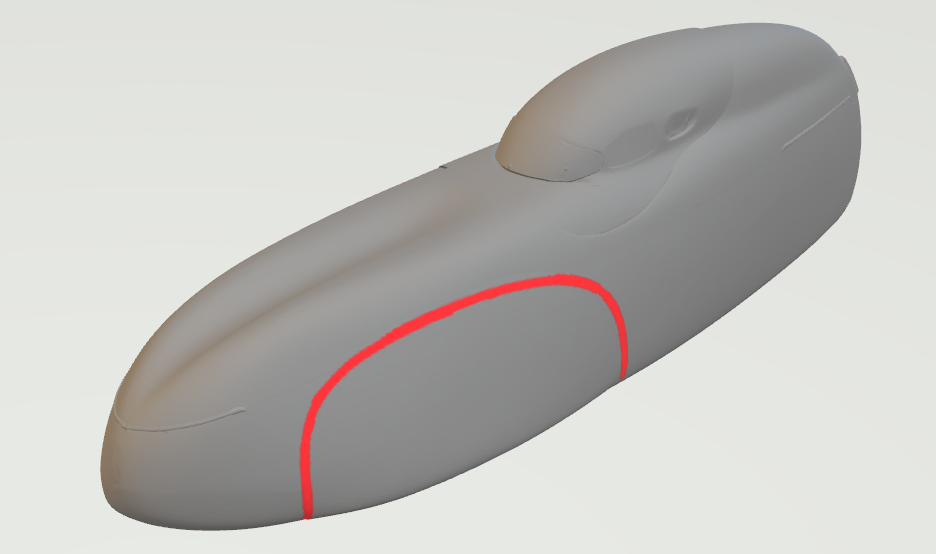
\includegraphics[width=.8\linewidth]{bilder/velo_wheelcase}
	\caption{Radkasten des Velomobils}
	\label{fig:wheelcase}
\end{figure}

Die erste Problemdomäne stellt die Optimierung der Radkästen eines Velomobils dar.
Da die momentanen Radkästen den Lenkausschlag des Velomobils erheblich einschränken, besteht das Ziel hierbei Radkästen zu generieren, die den maximalen, oder zumindest einen weiteren Lenkausschlag als den momentan möglichen, ermöglichen und dabei trotzdem gute aerodynamische Eigenschaften aufweisen.
Es ist zu erwarten, dass eine zusätzliche Fokussierung auf ein zweites Ziel, mit einer Qualitätsabnahme des ersten Ziels verbunden ist.
Trotzdem ergibt die Einführung eines Constraints nur Sinn, wenn die Abnahme an Optimalität bezüglich des Primärziels gering genug ist um eine Zunahme an Optimalität bezüglich des Sekundärziels vertretbar zu machen.
Das Ziel besteht also darin Lösungen zu entwickelt, welche durch minimalen Fitnessverlust einen maximalen Constraintgewinn möglich machen.

\subsubsection{OpenFOAM}

\todo{snappyhexmesh config, simple foam, kovergenz nach 200 zeitschritten}

\subsubsection{Constraint}
\begin{figure}[h]
	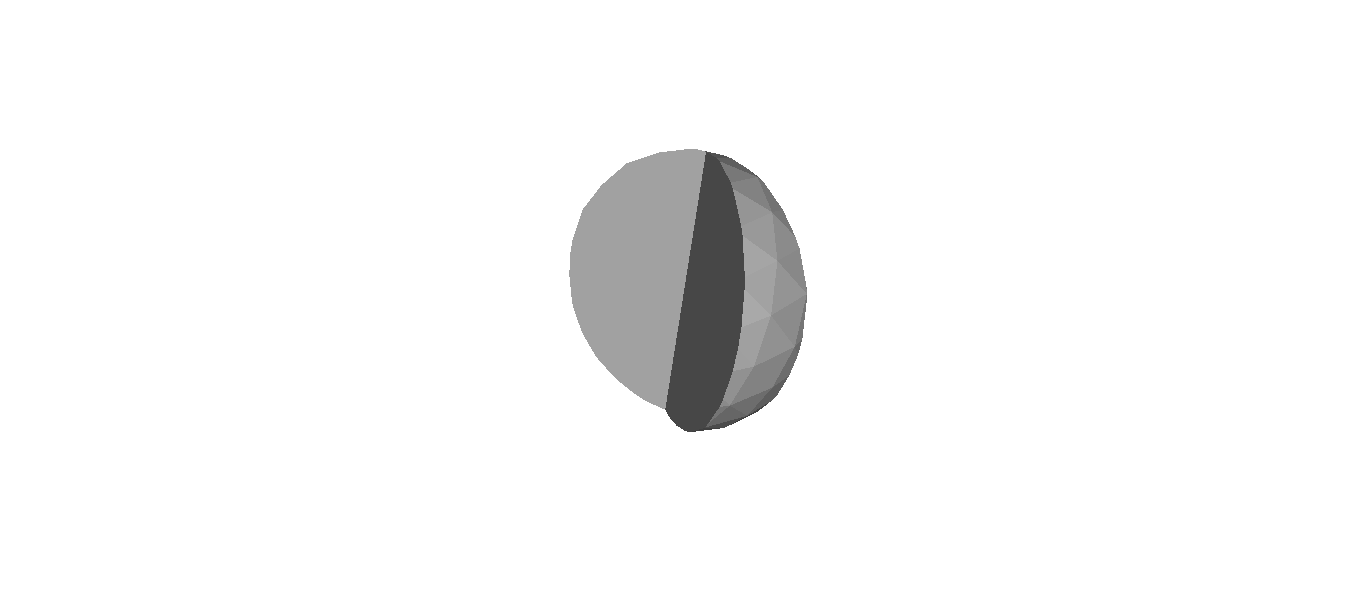
\includegraphics[width=.5\linewidth]{bilder/radausschlag.png}
	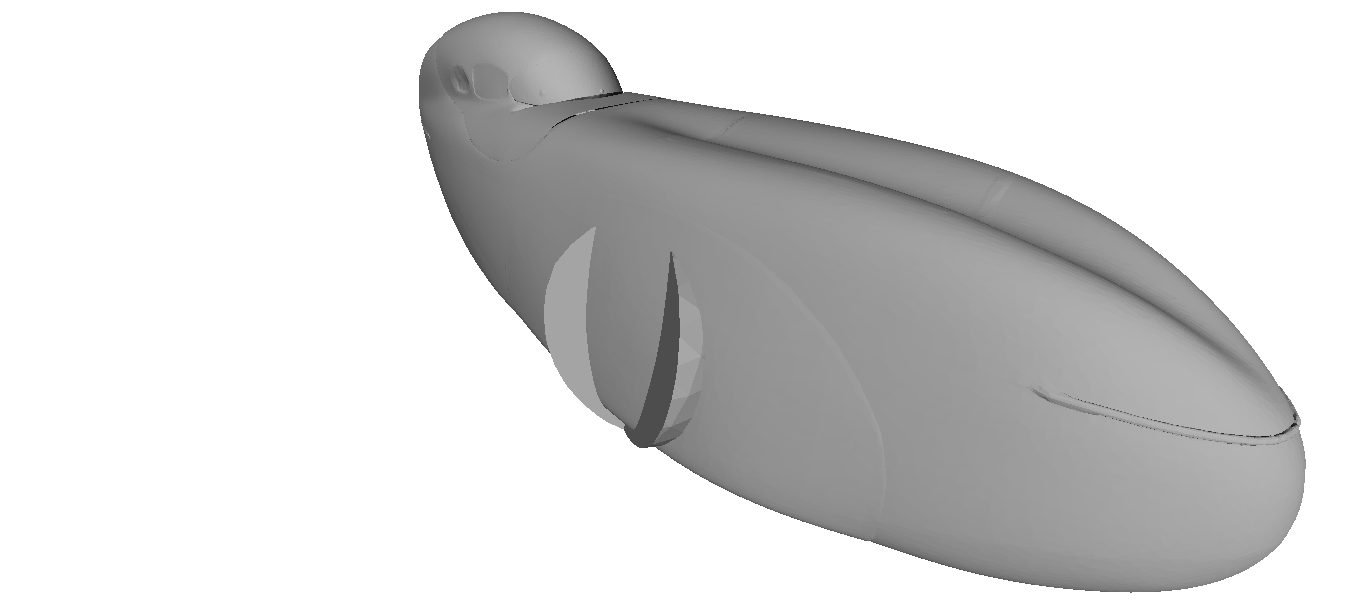
\includegraphics[width=.5\linewidth]{bilder/radausschlag_inclVelo.png}
	\caption{Das modellierte Radausschlagsvolumen}
	\label{fig:steering_volume}
\end{figure}
Zur Erfüllung des Constraints wurden alle möglichen Radausschläge als Volumen modelliert.
Dafür wurden aus einer Kugel entsprechend der maximalen Radausschlags nach rechts und links ein dreieckiges Stück ausgeschnitten.
Zusätzlich wurde die innere Hälfte der Kugel entfernt, da dort keine Überschneidungen stattfinden, und durch deren Entfernen, Berechnungen mit dieses Volumen effizienter sind.
Dieses Volumen ist in Abb. \ref{fig:steering_volume} alleine, in Abb. \ref{fig:steering_volume_with_velo} zusammen mit dem restlichen Velomobil zu sehen.
Es ist klar zu Erkennen, dass dieses Volumen die unverformten Radkästen schneidet, da diese den maximalen Lenkausschlag nicht ermöglichen.
 

\begin{table}[h]
	\begin{tabularx}{.5\textwidth}{ll}\hline
		
		Position & \\
		\hline
		x &	$926mm$ \\
		y &	$343mm$ \\
		z &	$205mm$	\\
	\end{tabularx}
	\begin{tabularx}{.5\textwidth}{ll}\hline
		Rotation & \\ \hline
		$\phi$ & $16,6\degree$ \\
		$\theta$ & $0\degree$ \\
		$\psi$ & $0\degree$ \\
	\end{tabularx}
	\begin{tabularx}{.5\linewidth}{ll}
		Radius des Rads & $230mm$ \\
		Radausschlag & $\pm24,37\degree$\\
		
	\end{tabularx}

\label{tab:wheel_params}
\caption{Parameter Radausschlag. Urpsprung des Koordinatensystems für Position auf Boden an der Spitze des Velomobils. Linkshändiges Koordinatensystem mit z Höhenachse und Velomobil in -x-Richtung ausgerichtet}
\end{table}

\begin{figure}[h]
	\centering
	
\includegraphics[width=.5\linewidth]{bilder/difference.png}
	\caption{Das Differenzvolumen für den unverformten Radkasten. Aus diesem wird der Strafwert berechnet}
	\label{fig:diff_volume}
\end{figure}
Da ein Ziel darin bestand, den Constraint nicht als binäres, erfüllt/nicht erfüllt Problem zu definieren, da zwischen zwei Lösungen, die den Constraint nicht erfüllen trotzdem qualitative Unterschiede bestehen können wie stark der Constraint verletzt wird, wird als Constraint das Differenzvolumen des Radausschlags minus verformten Radkastens gewählt.
Da alle generierten Verformungen der Radkästen symmetrisch sind, wird der Constraint jeweils nur für den rechten Radkasten berechnet.
Zwar besteht keine direkte Kausalität zwischen diesem Volumen und dem maximalen möglichen Radausschlag aber die Vermutung, dass eine geringeres Volumen dieser Differenz mit größerem möglichen Radausschlag korreliert ist liegt nahe.
Zur Berechnung der Differenz zwischen Radausschlagsvolumen und Radkasten wird die Bibliothek \textit{gptoolbox} \cite{gptoolbox.b} genutzt, zur Generierung von Tetraedermeshes zur Volumenberechnung \textit{TetGen} \cite{Si.2015}.
Ein Beispiel des Differenzvolumens zur Constraintberechnung ist in Abb. \ref{fig:diff_volume} zu sehen.
Dieses Volumen stellt die Differenz des Radausschlagvolumens und des unverformten Radkastens dar.
Um eine Differenz berechnen zu können wurde der rechte Radkasten geschlossen.
Da die Constraintberechnung in jeder Generation für jedes Kind erfolgen muss wurde der Radkasten außerdem vereinfacht um die Berechnung  des Constraints ausreichend schnell durchführen zu können.
Aus dem Volumen wird dann der Strafwert berechnet der in Relation zum Differenzvolumen des unverformten Radkastens
\footnote{Für den unverformten Radkasten beträgt das Differenzvolumen ca. $1,6L$} gesetzt wird.

Da sich der Constraint durch die Vereinfachung des Radkastens ausreichend schnell berechnen ließ, dass eine direkte Berechnung dessen für jedes Individuum zeitlich möglich war, wurde dies getan.
Das Trainieren eines zweiten Surrogatmodells zur Modellierung des Constraints hätte einen nicht unerheblichen Komplexitätszuwachs bedeutet , der an dieser Stelle nicht nötig war.
Also wurde dieser Strafwert direkt in die Fitnessfunktion integriert und als $\frac{V_{verformt}}{V_{unverformt}} * w_{constraint}$ auf die Fitness jedes Individuums addiert
\footnote{Die vorliegende SAIL-Implementation minimiert}.
Allerdings wurde der Strafwert zusätzlich noch in die Akquisefunktion, mit der einnerhalb von SAIL die Akquisekarte zur Auswahl neuer Individuen zur Auswertung stattfindet auf die gleiche Weise integriert. Das hat den Grund, dass das Gaußprozessmodell in solchen Bereichen bevorzugt Exploitation durchführen soll, die sowohl bezüglich der Aerodynamik, als auch bezüglich des Constraints eine gewisse Optimalität aufweisen, da genau in diesen Bereichen, in der finalen Auswertung von MAP-Elites solche Lösungen zu erwarten sind die bezüglich der Kombination dieser beiden Kriterien optimal sind.


\subsubsection{Wahl der Features}
%Die Kategorisierung wird von der \path{wheelcase_Categorize.m} verwaltet.

Als erste Kategorie wurde die Breite des Velomobils gewählt.
Diese Kategorie wurde deshalb gewählt, da hier sehr klare Hypothesen aufgestellt werden können, wie die Breite des Velomobils mit der Aerodynamik und dem Constraint interagiert.
Die erste Hypothese, die aufgestellt werden kann ist, dass breiteren Velomobilen die Erfüllung des Constraints leichter fällt. Es wäre also zu erwarten, dass breitere Velomobile den Constraint tendenziell besser erfüllen, als schmalere.
\begin{itemize}
	\item Breitere Velomobile sind positiv mit Erfüllung des Constraints korreliert.
\end{itemize}
Auch kann die Hypothese aufgestellt werden, dass die Breite negativ mit dem Luftwiderstandsbeiwert korreliert ist.
\begin{itemize}
	\item Breitere Velomobile sind negativ mit Luftwiderstandsbeiwert korreliert.
\end{itemize}
Insgesamt wäre also zu vermuten, dass entlang dieser Achse der Luftwiderstandsbeiwert zunimmt während der Strafwert des Constraints abnimmt.
%Der Test ob diese Erwartungen erfüllt sind stellt eine einfache Möglichkeit zur semantischen Verfifizierung der Ergebnisse dar.

Als zweite Kategorie wurde die x-Koordinate des breitesten Punkts gewählt.
Da das Velombil in negative x-Richtung ausgerichtet ist, bedeuten kleinere Werte hier, dass der Punkt weiter vorne liegt, größere, dass er weiter hinten liegt.
Zu dieser Kategorie lassen sich keine so direkten Hypothesen aufstellen wie zur ersteren.
Die Frage ob sich hier klare Tendenzen bezüglich den aerodynamischen Eigenschaften und/oder des Constraints aufzeigen ist auch ein Ziel der Untersuchung.

Da auch die Kategorisierung so häufig stattfindet, wird auch diese mit dem für die Berechnung des Constraints vereinfachten Modell des Radkastens durchgeführt. 
Dies stellt keinen signifikanten Verlust an Genauigkeit in der Kategorisierung dar, da sich die am feinsten gemeshten Teile des Radkastens an dessen Rändern befinden.
Gerade die sind aber die Teile des Radkastens, die am unwahrscheinlichsten den breitesten Punkt darstellen.
Auch führen minimale Genauigkeitsfehler in der Kategorisierung nicht dazu, dass die von MAP-Elites geforderte Lokalität verletzt wird.
Der Geschwindigkeitsgewinn bei der Berechnung hingegen mach es möglich solche Kategorien, für die eine Verformung des Radkastens notwendig ist, zu wählen, was in Relation einen wesentlich größeren Gewinn darstellt.

%\subsection{E-Roller}
%\label{sub:method_escooter}
%\missingfigure{E-Rollerbauteil}
%
%Die zweite Problemdomäne ist die explorative Untersuchung eines Bauteils an der Unterseite eines E-Rollers.
%Hier besteht die Frage ob nicht-triviale Bauteile aerodynamische Vorteile bieten, und welche Eigenschaften solche Bauteile aufweisen.
%
%\subsubsection{Setup}
%\subsubsection{OpenFOAM}
%\subsubsection{Constraint}
%\subsubsection{Wahl der Features}







%%%%%%%%%%%%%%%%%%%%%%%%%%%%%%%%%%%%%%%%%%%%%%%%%%
% Auswertung                                     %
%%%%%%%%%%%%%%%%%%%%%%%%%%%%%%%%%%%%%%%%%%%%%%%%%%
\newpage
\section{Auswertung}

\subsection{Radkasten}

\subsubsection{1. Experiment}

\begin{figure}[h]
	\centering
	\begin{tabularx}{.75\textwidth}{ll}\hline
		Anzahl initialer Samples & 100 \\
		Anzahl Samples & 500 \\
		Anzahl neuer Samples pro Akquiseschleife & 20 \\
		Anzahl Generationen Akquise-MAP-Elites & 1024 \\
		Kinder pro Generation Akquise-MAP-Elites & 32 \\
		Anzahl Generationen Ergebnis-MAP-Elites & 2048 \\
		Kinder pro Generation Akquise-MAP-Elites & 32 \\
		Auflösung der MAP-Elites Karte & 25 * 25  \\
		\hline
		Freiheitsgrade & 6 \\
		Mittelwertgewichtung & 1 \\
		Varianzgewichtung & 2 \\
		Constraintgewichtung & 1 \\
	\end{tabularx}
	\caption{Parametrisierung des ersten Experiments}
	\label{tab:param1st}
\end{figure}

Das Primärziel des ersten Experiments bestand darin zu verifizieren, dass der Algorithmus trotz Einbindung des Constraints korrekt funktioniert, d h. auch mit Constraint vergleichbare Werte bezüglich Luftwiderstandskoeefizienten erreicht werden, und der Algorithmus trotz des Constraints korrekt lernt.
Deshalb wurde die Parametrisierung vergleichsweise einfach gewählt, FFD-Deformationen fanden in zwei Punkten, in jeweils drei Richtungen statt.
\missingfigure{FFD-Deformationspunkte}
Auch wurde die Laufzeit soweit beschränkt, dass sinnvolle Aussagen darüber getroffen werden können, ob und wie gut der Algorithmus lernt, für finale Ergebnisse hingegen wäre die Anzahl an Samples die ausgewertet werden sowie die Anzahl an Genrationen für Akquise, und finaler Auswertung höher zu wählen.
Um bewerten zu können ob die Einbindung des Constraints einen Effekt auf den Algorithmus hat, und um diesen Effekt quantifizieren zu können wurde der Algorithmus unter den in Tabelle \ref{tab:param1st} beschriebenen Parametern sowohl mit Constraint als auch ohne Constraint durchgeführt. 
\begin{figure}[h]
	
	\centering
	\begin{minipage}{0.45\textwidth}
		\centering
		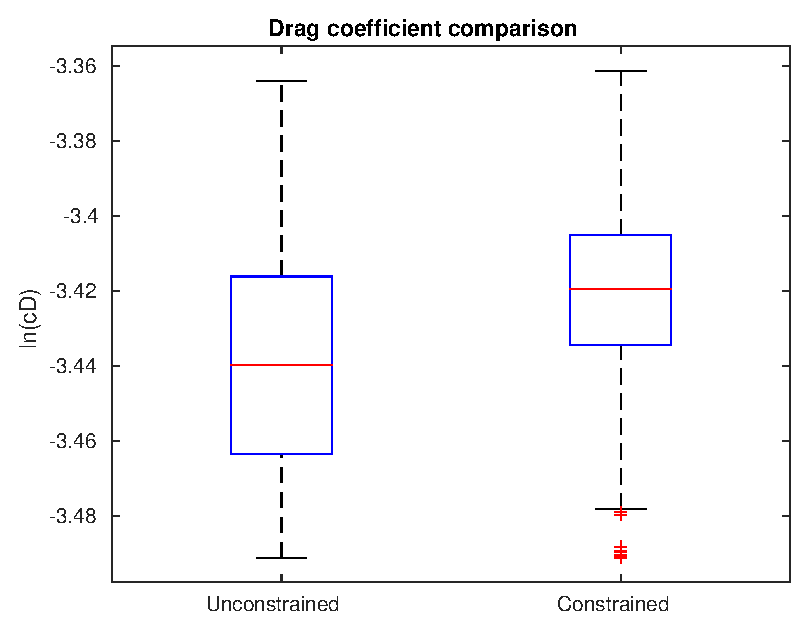
\includegraphics[width=1\linewidth]{bilder/2pt500Samples/dragBoxplot}
		\caption{Comparison of final drag values}
		\label{fig:1stdragbox}
	\end{minipage}\hfill
	\begin{minipage}{0.45\textwidth}
		\centering
		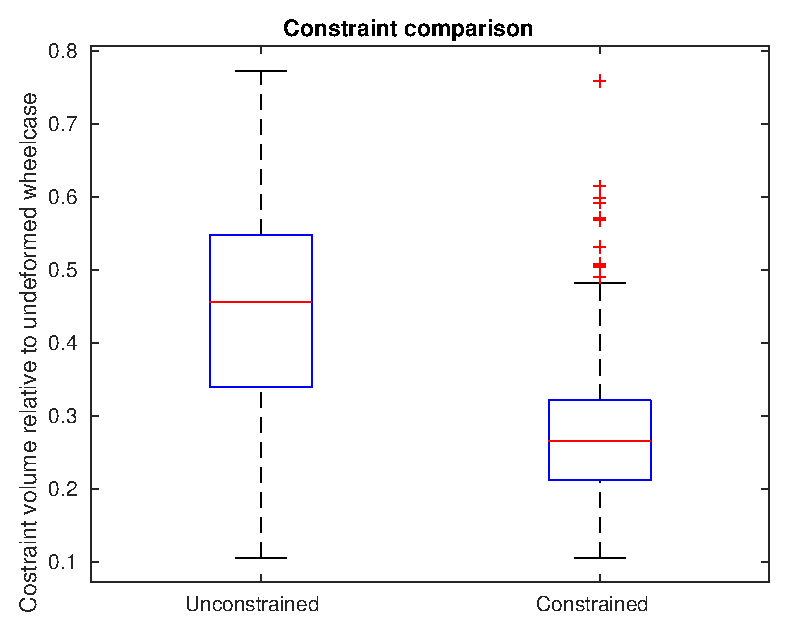
\includegraphics[width=1\linewidth]{bilder/2pt500Samples/constraintBoxplot}
		\caption{Comparison of final constraint values}
		\label{fig:1stconbox}
	\end{minipage}
\end{figure}

Die Ergebnisse des ersten Experiments sehen vielversprechend aus In Abb. \ref{fig:1stdragbox} ist ein Vergleich der Luftwiderstandsergebnisse 
\footnote{Im Experiment wurde statt der direkten Luftwiderstandswerte, der natürliche Logarithmus dieser genutzt.} 
der erzeugten Lösungen abgebildet.
Die erste Beobachtung die gemacht werden kann, ist dass die produzierten Werte aus der Variante mit Constraint in der gleichen Größenordnung liegen wie die aus der Variante ohne Constraint.
Der Algorithmus scheint also auch mit Constraint noch korrekt zu lernen.
Es ist zu Erkennen, dass die Einbindung des Constraints zu einer Verschlechterung der Luftwiderstandswerte führt, eine Verschlechterung dieser durch eine Fokussierung auf zwei Ziele ist allerdings zu erwarten.
Trotzdem muss betont werden, dass die Verschlechterung erstaunlich klein ist, so beträgt der relative Unterschied zwischen dem Median der Version mit Constraint und dem Median der Version ohne nur \todo{genaue zahl}.

Um eine solche Verschlechterung zu rechtfertigen sollte die Qualität des Sekundärziels herangezogen werden.
Dazu ist in \ref{fig:1stconbox} ein Vergleich bezüglich des Constraintvolumens dargestellt.
Die erste Beobachtung hier ist, dass die Einbindung des Constraints zu einer stärkeren Beachtung dessen führt.
Das ist offensichtlich das Ziel bei der Nutzung eines Constraints, dass diese Erwartung erfüllt wird zeigt, dass die Formulierung des Constraints insofern korrekt ist, dass eine Verbesserung dieses erreicht werden kann.
Auch ist hervorzuheben, dass die relative Verbesserung des Constraints wesentlich stärker ist als die relative Verschlechterung des Luftwiderstands.
Eine Verschlechterung des Medians bezüglich des Luftwiderstands von \todo{genaue zahl} geht hier mit einer Verbesserung des Medians bezüglich des Constraints von \todo{genaue zahl} einher.

Interessant sind auch die Grenzen der Verteilungen, beide Verteilungen weisen eine untere Grenze von ca. 0.1, sprich 10\% des Außenvolumens des unverformten Radkastens auf.
Dies lässt sich dadurch erklären, dass das Radausschlagsvolumen einen Teil unterhalb des Radkastens hat, der durch eine seitliche Deformation des Radkastens nicht eliminiert werden kann.
Die zweite interessante Grenze stellt die Obergrenze von 0.8 dar.
Selbst die schlechteste Lösung in der Version ohne Constraint ist damit besser als der undeformierte Radkasten.
Dies kann einerseits an zu eng gewählten Deformationsparametern liegen, die genutzte Konfiguration erlaubte allerdings Deformationen nach innen.
Die plausiblere Hypothese ist, dass die Wahl der Breite des Radkastens als Feature bedeutet, dass eine Minimalbreite existiert, bei der nicht das Zentrum des Radkastens, sondern die Ränder den breitesten Punkt darstellen.
Jede Deformation die das Zentrum stärker nach innen verformt, würde in die gleiche Zelle der Karte eingeordnet werden.
Wenn weniger stark verformte Radkästen bezüglich deren Fitness optimaler sind, wird dies dazu führen, dass Radkästen mit einer stärkeren Verformung nach innen keinen Einzug in die Karte finden können.

Aufgrund der Tatsache, dass SAIL ein divergenter Optimierungsalgorihtmus ist haben die finalen Verteilungen nur eingeschränkte Aussagekraft.
Besonders dadurch, dass das Feature der Breite des Velomobils mit der Schwierigkeit der Erfüllung des Constraints korreliert ist, müssen auch die produzierten Karten analysiert werden.

\begin{figure}[h]
	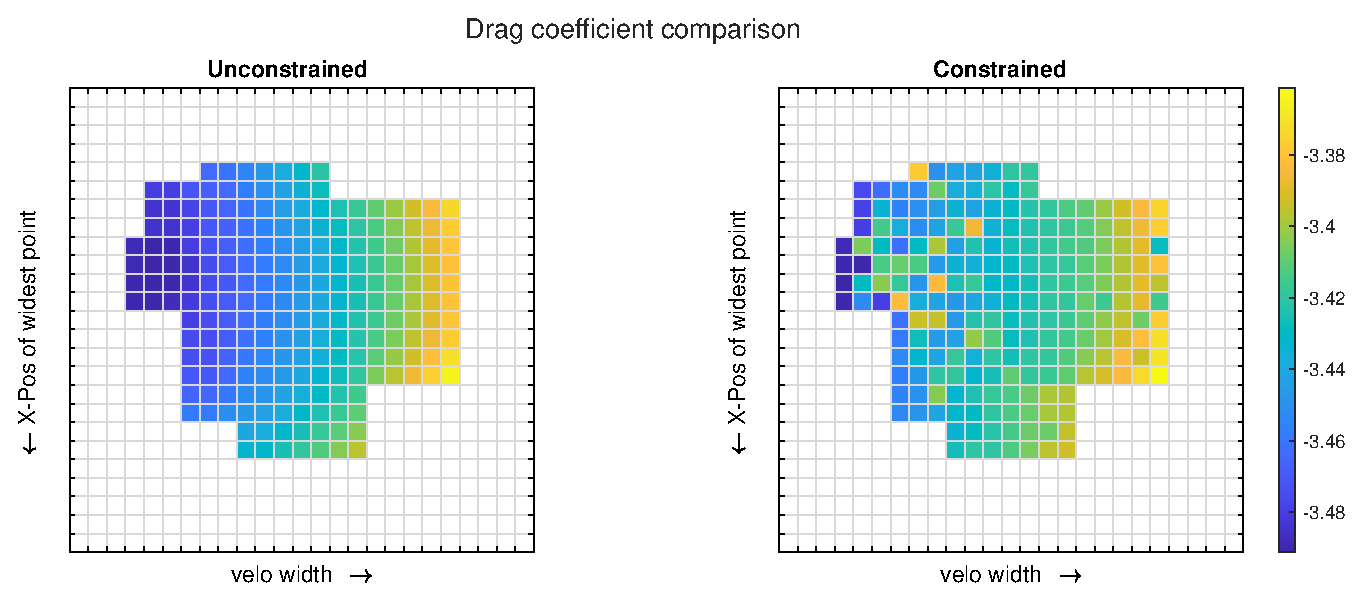
\includegraphics[width=1\linewidth]{bilder/2pt500Samples/dragMapComparison}
	\caption{Maps of final drag values}
	\label{fig:1stmapDrag}
\end{figure}

In Abb. \ref{fig:1stmapDrag} sind die Karten von Luftwiderstandskoeffizienten der produzierten Ergebnisse in beiden Versionen aufgeführt.
Die Karte ohne Constraint bestätigt die Hypothese, dass breitere Velomobile mit schlechterem Luftwiderstandskoeffizienten korreliert sind.
Auch ist erkennbar, dass es ein mittleres Optimum bezüglich der x-Position dieses Punktes zu geben scheint, da Luftwiderstandswerte sowohl bei Abweichungen nach oben als auch bei Abweichungen nach unten schlechter werden.
Dass die oben aufgestellte Hypothese bestätigt werden kann und die Karte einen graduellen Verlauf aufweist, sind Zeichen für die korrekte Funktionalität des Algorithmus.
Im Gegensatz dazu ist die Karte der Variante mit Constraint wesentlich unregelmäßiger.
Dies bedeutet allerdings nicht, dass der Algorithmus in dieser Variante nicht korrekt arbeitet, die Unregelmäßigkeit der Karte rührt daher, dass die Fitness des Algorithmus aus einer Kombination von Luftwiderstandskoeffizienten und Constraint zusammensetzt.
Auch bewegen sich die Luftwiderstandswerte, wie bereits anhand der Boxplots sichtbar war im Bereich.
Besonders gute Lösungen bezüglich einer dieser beiden Komponenten können fehlende Optimalität bezüglich der anderen damit ausgleichen.
Trotzdem sind auch in dieser Karte die gleichen zugrundeliegenden Tendenzen zu erkennen, breitere Velomobile sind auch hier schlechter bezüglich des Luftwiderstands sind und Optimalität sinkt nach unten und oben.
Interessant ist, dass am rechten, sprich breiteren, Ende einige Lösungen gefunden wurden die sogar bessere Luftwiderstandswerte aufweisen als deren Gegenstücke in der Variante ohne Constraint.
Und auch wenn auf der linken Seite einige Lösungen existieren, welche erheblich schlechtere Luftwiderstandswerte aufweisen wie ihre Gegenstücke, so existieren auch sehr viele mit vergleichbaren Werten.
Um solche Verschlechterungen in Kontext setzten zu können müssen sich die Karten des Constraints angeschaut werden.

\begin{figure}[h]
	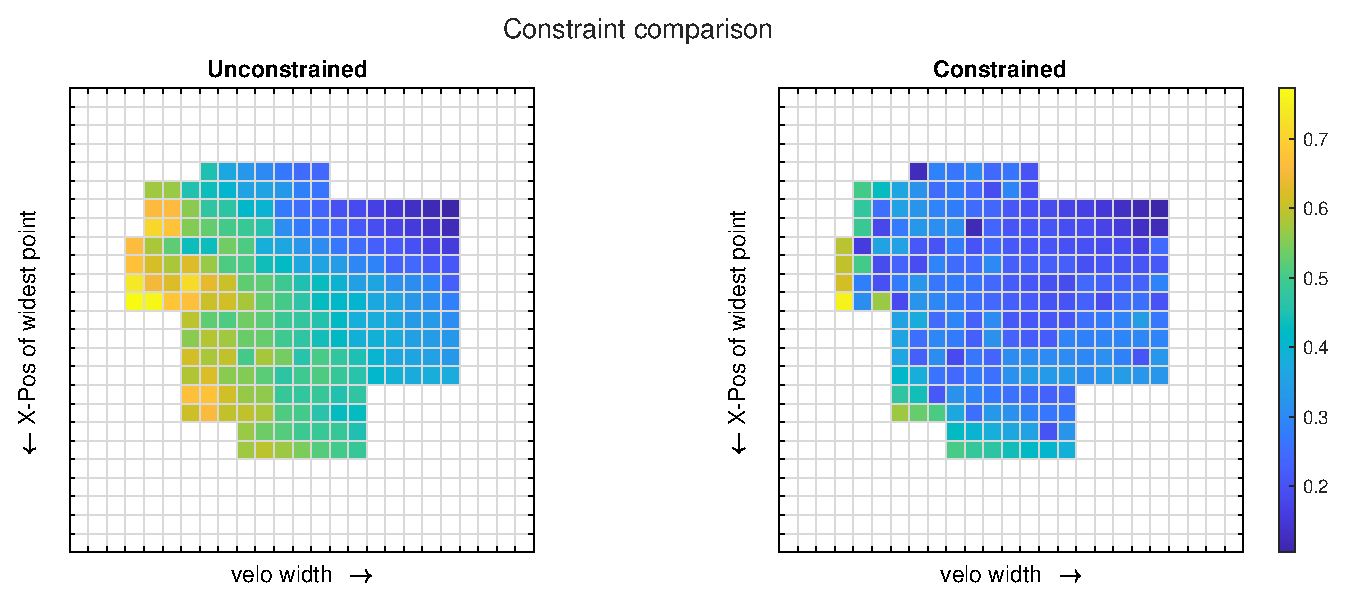
\includegraphics[width=1\linewidth]{bilder/2pt500Samples/constraintMapComparison}
	\caption{Maps of final constraint values}
	\label{fig:1stmapCon}
\end{figure}

In Abb. \ref{fig:1stmapDrag} sind die Karten der korrespondierenden Constraint-Werte für beide Varianten zu sehen.
Ersteinmal lässt sich auch hier die Hypothese bestätigen, dass breitere Velomobile den Constraint besser erfüllen.
Interessant ist allerdings auch, dass ohne Einbindung des Constraints, Lösungen, deren breitester Punkt weiter vorne ist den Constraint besser erfüllen.

Im Vergleich der beiden Karten ist noch viel stärker, als den Boxplots, ersichtlich welchen Effekt die Einbindung des Constraints hat.
Es ist klar ersichtlich wie viel besser ein Großteil der Lösungen den Constraint erfüllen.
Besonders stark is dieser Effekt im Mittelfeld der Karte in denen sich Constraintwerte halbieren und teilweise noch stärker verringern.
Zum rechten extremen Rand schwächt die Constraintverbesserung ab, da dortige Radkästen so breit sind, dass selbst die Variante ohne Constraint diesen leicht erfüllen kann.
Auch ist hervorzuheben, dass sich Verbesserungen bis zum linken Rand der Individuen durchziehen.
Selbst in der linken, sprich schmalsten Spalte, ist eine Verbesserung der Individuen erkennbar, und die nächste Spalte enthält bereits ein Individuum welches nahe der besten gefundenen Constraint-Werte angesiedelt ist.

\begin{figure}[h]
	\centering
	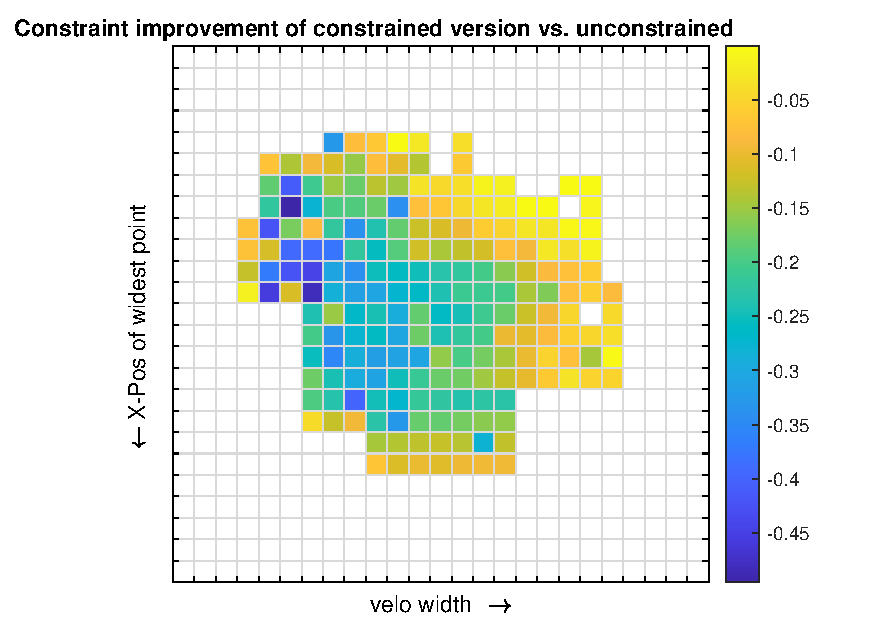
\includegraphics[width=.7\linewidth]{bilder/2pt500Samples/constraintImprovements}
	\caption{Maps of final constraint values}
	\label{fig:1stmapConCompare}
\end{figure}

In Abb. \ref{fig:1stmapConCompare} ist die Verbesserung der Constraintwerte von der Version ohne Constraint zur Version mit Constraint dargestellt.
Der bereits oben erwähnte Effekt, dass die größten Verbesserungen besonders in der linken Hälfte der Karte stattfinden ist hier noch klarer ersichtlich.
Gerade diese Hälfte ist allerdings die, die bessere Luftwiderstandswerte aufweist und in der die Erfüllung des Constraints aufgrund der geringeren Breite, die Velomobile in diesen Zellen auszeichnet, wesentlich schwerer fällt.
\missingfigure{Einige Deformationen}
Zusammenfassend kann man sagen, dass die Einbindung des Constraints mit den im ersten Experiment vorliegenden Einschränkungen merkliche Auswirkungen auf das Ergebnis hat.
Auch ist herauszustellen, dass eine starke Verbesserung des Constraints bei einer schwachen Verschlechterung des Luftwiderstands stattfindet.
%Weiterführenden Experimente sollten ohne die Einschränkungen bezüglich Freiheitsgraden und Länge des Experimentes

\subsubsection{2. Experiment}

Mit dem ersten Experiment konnte gezeigt werden, dass der Algorithmus sowohl Luftwiderstandskoeffizienten als auch Constraint optimiert, und dabei relativ geringe Kosten in Bezug zum erreichten Luftwiderstand entstehen.
Das erste Experiment hatte allerdings einige Einschränkungen, bezüglich der Parametrisierung um es einfach zu halten.
Die erste dieser Einschränkungen war die Reduzierung auf Deformation in 2 Punkten, sprich 6 Freiheitsgraden.
Diese Reduzierung half dabei das Problem klein zu halten, hatte aber eine erhebliche Einschränkung des Lösungsraums zur Folge.
Ziel des zweiten Experiments ist es die Anzahl an Freiheitsgraden erheblich zu erhöhen, damit die Zahl an möglichen Deformationen erheblich zu erhöhen, was den positiven Effekt der Einbindung eines Constraints hoffentlich erhöht.
Dazu wird die Anzahl an Deformationspunkten auf 6 erhöht, wodurch sich 18 Freiheitsgrade ergeben.
\missingfigure{FFD-Deformationspunkte}

\begin{figure}[h]
	\centering
	\begin{tabularx}{.75\textwidth}{ll}\hline
		Anzahl initialer Samples & 100 \\
		Anzahl Samples & 500 \\
		Anzahl neuer Samples pro Akquiseschleife & 20 \\
		Anzahl Generationen Akquise-MAP-Elites & 1024 \\
		Kinder pro Generation Akquise-MAP-Elites & 32 \\
		Anzahl Generationen Ergebnis-MAP-Elites & 2048 \\
		Kinder pro Generation Akquise-MAP-Elites & 32 \\
		Auflösung der MAP-Elites Karte & 25 * 25  \\
		\hline
		%\rowcolor{lightgray}
		Freiheitsgrade & 18 \\
		Mittelwertgewichtung & 1 \\
		Varianzgewichtung & 2 \\
		Constraintgewichtung & 1 \\
	\end{tabularx}
	\label{tab:param2nd}
	\caption{Parametrisierung des zweiten Experiments (Änderungen zum ersten Experiment hervorgehoben)}
\end{figure}

\begin{figure}[h]
	
	\centering
	\begin{minipage}{0.45\textwidth}
		\centering
		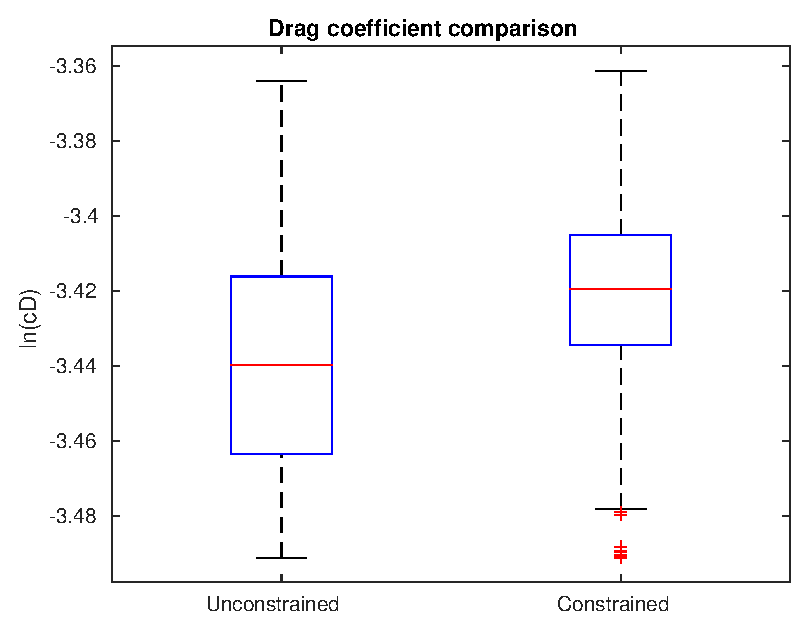
\includegraphics[width=1\linewidth]{bilder/2pt500Samples/dragBoxplot}
		\caption{Comparison of final drag values}
		\label{fig:1stdragbox}
	\end{minipage}\hfill
	\begin{minipage}{0.45\textwidth}
		\centering
		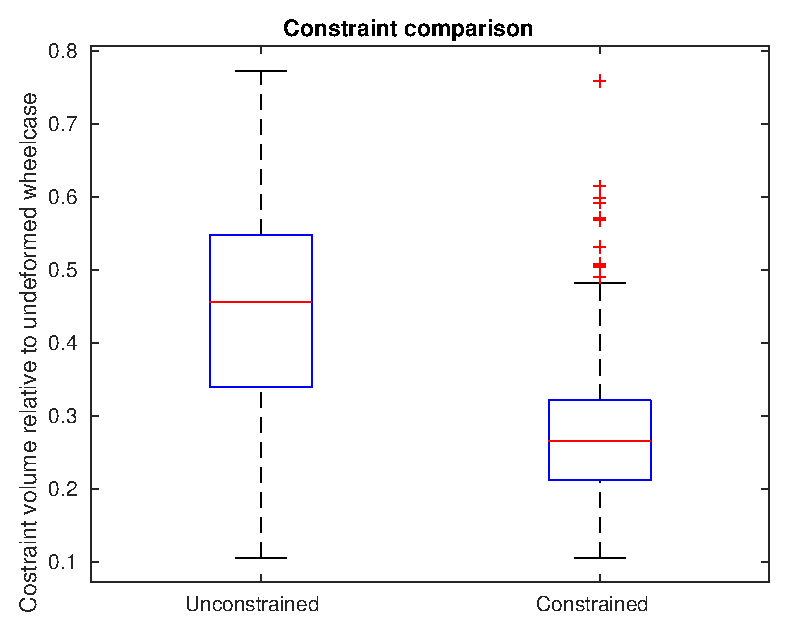
\includegraphics[width=1\linewidth]{bilder/2pt500Samples/constraintBoxplot}
		\caption{Comparison of final constraint values}
		\label{fig:1stconbox}
	\end{minipage}
\end{figure}

\subsubsection{3. Experiment}

Das zweite Einschränkung des ersten Experiments war die Beschränkung auf eine kleinere Anzahl an ausgewerteten Samples und Generationen in Akquise- und Ergebnis-MAP-Elites.
Durch die Beschränkung auf eine kleinere Anzahl an Samples besteht die Möglichkeit, dass der Suchraum nicht präzise genug und/oder nicht weitläufig genug abgebildet wurde.
Die Beschränkung in Generationen des Akquise- und Ergebnis-MAP-Elites kann dazu führen, dass diese noch nicht vollständig auskonvergiert sind.
Da die Überlegung nahe liegt, dass die Variante mit Constraint länger benötigen könnte um auszukonvergieren, sollte untersucht werden ob die Erhöhung dieser Parameter zu signifikanten Änderung im Vergleich zur kürzeren Version führt, indem die Gewinne nach 500 Samples und 1024 bzw. 2018 Generationen quantifiziert werden.

\begin{figure}[h]
	\centering
	\begin{tabularx}{.75\textwidth}{ll}\hline
		Anzahl initialer Samples & 100 \\
		%\rowcolor{lightgray}
		Anzahl Samples & 1000 \\
		Anzahl neuer Samples pro Akquiseschleife & 20 \\
		%\rowcolor{lightgray}
		Anzahl Generationen Akquise-MAP-Elites & 2048 \\
		Kinder pro Generation Akquise-MAP-Elites & 32 \\
		%\rowcolor{lightgray}
		Anzahl Generationen Ergebnis-MAP-Elites & 4096 \\
		Kinder pro Generation Akquise-MAP-Elites & 32 \\
		Auflösung der MAP-Elites Karte & 25 * 25  \\
		\hline
		Freiheitsgrade & 18 \\
		Mittelwertgewichtung & 1 \\
		Varianzgewichtung & 2 \\
		Constraintgewichtung & 1 \\
	\end{tabularx}
	\label{tab:params3rd}
	\caption{Parametrisierung des dritten Experiments (Änderungen zum zweiten Experiment hervorgehoben)}
\end{figure}

\subsubsection{Zusammenfassung}


\subsection{E-Roller}
\subsubsection{Experimente}
\subsubsection{Analyse}
\subsubsection{Zusammenfassung}


%\begin{figure}
%	\begin{tabularx}{.75\textwidth}{ll}\hline
%		Anzahl initialer Samples &  \\
%		Anzahl Samples &  \\
%		Anzahl neuer Samples pro Akquiseschleife & \\
%		Anzahl Generationen Akquise-MAP-Elites & \\
%		Kinder pro Generation Akquise-MAP-Elites & \\
%		Anzahl Generationen Ergebnis-MAP-Elites & \\
%		Kinder pro Generation Akquise-MAP-Elites &  \\
%		Auflösung der MAP-Elites Karte &   \\
%		\hline
%		Freiheitsgrade &  \\
%		Mittelwertgewichtung & 1 \\
%		Varianzgewichtung & 2 \\
%		Constraintgewichtung & 1 \\
%	\end{tabularx}
%\end{figure}


%%%%%%%%%%%%%%%%%%%%%%%%%%%%%%%%%%%%%%%%%%%%%%%%%%
% Zusammenfassung                                %
%%%%%%%%%%%%%%%%%%%%%%%%%%%%%%%%%%%%%%%%%%%%%%%%%%
\newpage
\section{Diskussion}

\subsection{Radkasten}

\subsection{E-Roller}

Für den E-Roller wurde in dieser Arbeit nur ein Experiment durchgeführt.
Aus dessen Ergebnisse können trotzdem einige Schlussfolgerungen gezogen werden.

Zuerst muss klargestellt werden, dass  die berechneten Lösungen aufgrund der Unsicherheit, die mit der Korrektheit der Openfoam-Simulationen zusammenhängt, nicht als absolute Wahrheit behandelt werden dürfen.
Alle Beobachtungen, die auf Basis dieses Experiments getätigt wurden, benötigen weitere Verifikation der Korrektheit der Simulationen.
Trotzdem können einige Dinge an diesem Experiment analysiert werden und für eventuelle zukünftige Experimente genutzt werden.

Die erste Beobachtung, die an diesem Experiment gemacht werden konnte, ist, dass die Anwendung von SAIL auf diese Problemdomäne möglich ist.
Es konnte erfolgreich ein Surrogatmodell trainiert werden auf dessen Basis MAP-Elites durchgeführt werden konnte.
Es konnte eine Karte aus phänotypisch diversen Lösungen generiert werden, auch wenn diese Karte nur wenige Lösungsklassen enthielt.
Es kann nicht abschließend gesagt werden ob für das Problem nur Lösungen aus diesen Lösungsklassen brauchbar sind, oder ob die Limitierung auf diese Lösungsklassen ein Produkt der Konfiguration ist.
Auch ist es möglich, dass durch die Fehlkonfiguration von Openfoam Effekte, die nicht-triviale Lösungen haben könnten überhaupt nicht gemessen werden können, oder von der Stärke der Oszillation überdeckt werden.

Es konnte festgestellt werden, dass praktisch nur symmetrische Bauteile generiert wurden.
Damit konnte die Hypothese \todo{nummer}, dass symmetrische Bauteile für den symmetrischen E-Roller optimal sind bestätigt werden.

Es wurde grundsätzlich die Tendenz beobachtet, dass flachere Bauteile bessere Luftwiderstandswerte aufweisen.
Dieses Ergebnis ist zwar etwas ernüchternd, da die Hoffnung bestand außergewöhnliche Bauteile zu generieren, die bessere aerodynamischen Eigenschaften aufweisen, als ein sehr triviales.
Allerdings gilt wie bereits erwähnt, dass die Ungenauigkeit der Openfoam-Simulation kleine Effekte, die durch anders förmige Bauteile entstehen würden schlicht ignoriert.

\section{Ausblick}

\subsection{Radkasten}

In der Arbeit konnte gezeigt werden, dass eine Einbindung eines Constraints in ein divergentes Optimierungsverfahren möglich ist.

In der Arbeit wurden nur zwei FFD-Konfigurationen genutzt.
Die erste war sehr einfach um an dieser zu testen, dass der Algorithmus die richtigen Tendenzen aufzeigt.
Nachdem das erfolgt war wurde eine komplexere FFD-Konfiguration mit 18 Freiheitsgraden gewählt um mehr Deformationen zu erlauben.
Selbst diese erlaubt allerdings nur begrenzt viele Deformationen.
Es wäre sinnvoll die Anzahl an Freiheitsgraden weiter zu steigern und besonders auf die Punkte zu achten, die wichtig für Lösungen sind.
So wurde in der Arbeit festgestellt, dass Deformationen in y, wie erwartet sehr wichtig sind, aber auch, dass auch Deformationen in z wichtig sind.
Deformationen in x-Richtung waren weitergehend unwichtig und stellten damit Dimensionen dar, die keine interessanten zusätzlichen Deformationen erlaubten.
Es sollt also auch vermieden werden alle Punkte in allen Dimensionen zu deformieren und es sollte sich stattdessen auf y-Deformationen in allen und z-Deformationen in den oberen und unteren Rändern fokussiert werden.

Es könnte in Erwägung gezogen werden den Constraint statt Strafwert als Feature-Dimension aufzunehmen.
Dadurch würde die problematische Gewichtung zwischen Luftwiderstand und Strafwert wegfallen und es würde eine Diversität an Lösungen entlang der Constrainterfüllung generiert.
Dadurch würde garantiert, dass Lösungen verschiedener Constrainterfüllung generiert werden und es könnte eine Untersuchung stattfinden wo überhaupt Lösungen generiert werden, die den Constraint erfüllen, da diese nicht wie in der momentanen Version von aerodynamisch besseren Lösungen die den Constraint schlechter erfüllen verdrängt werden können.

Auch sollte über die Parametrisierung des Gaußprozesses nachgedacht werden.
Besonders die isotropische Kovarianzfunktion sollte gegen eine mit Automatic relevance determination ausgetauscht werden, da es denkbar ist, dass Dimensionen, die auf y-Deformationen abgebildet werden andere Längenmaße benötigen, als solche, die auf z-Deformationen abgebildet werden.

Die hier durchgeführten Experimente wurden mit einem vereinfachten Modell des Velomobils, welches die Räder nicht enthält, berechnet.
Da die Radkästen mit hoher Wahrscheinlichkeit Einfluss auf die Turbulenzen um die Räder des Velomobils haben werden, wären Experimente, die die Räder des Velomobils einschließen wünschenswert.

\subsection{E-Roller}

Aufgrund der Schwierigkeiten der Anwendung von SAIL auf die E-Rollerdomäne lag der Fokus der Untersuchung dieser Arbeit in der Radkastendomäne.
Das Hauptproblem der in dieser Arbeit erzeugten Ergebnisse ist die Unsicherheit bezüglich deren Korrektheit.
Der Grund dafür ist der Fakt, dass die cD-Werte in der gewählten Konfiguration OpenFoam nicht konvergierten.
Der Grund dafür kann eine fehlerhafte Parametrisierung Openfoams sein, die Anpassung dieser Konfiguration sprengt allerdings den Umfang dieser Arbeit.
In zukünftigen Untersuchungen sollte also, vor der Nutzung von SAIL, zuerst sichergestellt werden, dass die zugrundeliegende Simulation in Openfoam realitätsgetreue Ergebnisse liefert.
Ist das nicht garantiert können alle möglichen Ergebnisse von SAIL nur beschränkte Aussagekraft haben.

Des weiteren sind die erzeugten Formen für das Bauteil nicht besonders kreativ oder bahnbrechend.
Das kann daran liegen, dass für dieses Bauteil keine guten unintuitiven Lösungen existieren.
Die Anzahl an möglichen Lösungen wird allerdings durch die gewählte Deformationskonfiguration eingeschränkt.
Es sollte möglicherweise über andere FFD-Konfigurationen, beziehungsweise Deformatiormationen in anderen Punkten und/oder Richtungen nachgedacht werden.
Besonders, dass die seitlichen Ränder des Bauteils in der hier gewählten Konfiguration nicht deformiert werden können stellt eine starke Einschränkung dar.
Auch sollte in Erwägung gezogen werden die linke und rechte Hälfte symmetrisch zu verformen.
Erstens ist anzunehmen, dass dadurch, dass der E-Roller an sich symmetrisch ist die Strömungen die das Bauteil treffen ebenso symmetrisch sind.
Lösungen die in solchen Strömungen am besten abschneiden werden mit hoher Wahrscheinlichkeit symmetrisch sein.
Im Experiment konnte auch beobachtet werden, dass alle erzeugten Bauteile fast symmetrisch waren.
Alle Asymmetrien waren meist leicht und eher auf die Größe des genetischen Suchraums zurückzuführen, als auf einen Vorteil durch eine asymmetrische Bauart.
Auch ist fragwürdig ob  asymmetrische Bauteile überhaupt in die Designparameter des E-Rollers passen.
Ästhetik ist schwer quantifizierbar und Fertigungstauglichkeit sowie Einbettbarkeit des Bauteils in den E-Roller wurden in dieser Arbeit nicht untersucht, alle drei könnte aber von vornherein gegen asymmetrische Bauteile sprechen.
Durch die symmetrische Verformung des Bauteils könnte allerdings die Anzahl an benötigten Freiheitsgraden halbiert, beziehungsweise mit der gleichen Anzahl an Freiheitsgraden feinere Deformationen erlaubt werden.
In Anbetracht dieser drei Tatsachen scheinen symmetrische Verformungen bei denen die Verformungen der linken und rechten Hälfte des Bauteils aus dem gleichen Genom abgeleitet werden sinnvoller.

In dem durchgeführten Experiment waren die besten Ergebnisse bezüglich des Luftwiderstands solche die effektiv flach oder leicht nach oben deformiert waren.
Es besteht die Möglichkeit, dass nach oben deformierte Bauteile noch optimaler sind.
Dieser Lösungsraum sollte nach Lösungen untersucht werden.
Allzu stark deformiert Lösungen wurden in  dem durchgeführten Experiment durch die beschränkte minimale Deformation ausgeschlossen.
Es wäre möglich mehr Deformationen nach oben zu erlauben um solche Lösungen genauer zu untersuchen.
Zwar muss dann eine Möglichkeit gefunden werden, dass solche Bauteile, den restlichen E-Roller nicht schneiden, sodass beispielsweise um dessen Bauteile herum deformiert wird.
Dies könnte beispielsweise durch die Einführung eines Constraints geschehen, der testet, ob das Bauteil mit anderen Teilen des E-Rollers kollidiert.

Durch die Wahl des tiefsten Punkt als eines der Features war es selbst für leicht nach oben deformierte Bauteile schwer Einzug in die Karte zu erhalten.
Deshalb sollte zusätzlich über die die Kategorien zu nachgedacht werden, nach denen die Bauteile phänotypisch kategorisiert werden.
Die gewählten Kategorien wurden hauptsächlich aus dem Grund gewählt, dass diese einfach berechenbar und klar verständlich sind.
Es wäre vermutlich sinnvoll für die Domäne abgewägte Kategorien zu wählen, und zu untersuchen wie sich dies auf die Lösungen auswirkt.

Zuletzt stellte die benötigte Laufzeit für OpenFoam trotz der Nutzung des vereinfachten E-Roller Modells eine nicht unbeträchliche Hürde dar.
Dies ist vor allem auf die komplexere Form des E-Rollers im Vergleich zur aerodynamisch optimierten Projektilform des Velomobils und die längere Simulationsdauer von 1000 Sekunden zurückzuführen.
Eine qualitative Untersuchung welche Teile des E-Rollers wegrationalisiert werden können, ohne signifikante Ungenauigkeit in die Ergebnisse einzuführen, könnte die Laufzeit reduzieren wodurch beispielsweise wieder präzise Funktionsauswertungen ermöglicht werden, was mehr Freiheitsgrade erlauben kann.

%%%%%%%%%%%%%%%%%%%%%%%%%%%%%%%%%%%%%%%%%%%%%%%%%%
% Literaturverzeichnis                           %
%%%%%%%%%%%%%%%%%%%%%%%%%%%%%%%%%%%%%%%%%%%%%%%%%%
\newpage
% Literaturverzeichnis soll nicht nur Literatur heißen
\renewcommand\refname{Literaturverzeichnis}
\bibliography{Literaturverzeichnis}

%%%%%%%%%%%%%%%%%%%%%%%%%%%%%%%%%%%%%%%%%%%%%%%%%%
% Anhang                                         %
%%%%%%%%%%%%%%%%%%%%%%%%%%%%%%%%%%%%%%%%%%%%%%%%%%
%\newpage
%\section{Anhang}


%%%%%%%%%%%%%%%%%%%%%%%%%%%%%%%%%%%%%%%%%%%%%%%%%%
% Ende                                           %
%%%%%%%%%%%%%%%%%%%%%%%%%%%%%%%%%%%%%%%%%%%%%%%%%%
\end{document}
